\documentclass{article}
\usepackage[utf8]{inputenc}
\usepackage{array}
\usepackage{multirow}
\usepackage{graphicx}
\usepackage{color}   %May be necessary if you want to color links
\usepackage{hyperref}
\usepackage{longtable}
\usepackage{float}
\usepackage[table]{xcolor}
\usepackage{amssymb}
\usepackage{minted}
\setlength{\arrayrulewidth}{0.5mm}
\setlength{\tabcolsep}{18pt}
\renewcommand{\arraystretch}{2.5}
\hypersetup{
    colorlinks=false, %set true if you want colored links
    linktoc=all,     %set to all if you want both sections and subsections linked
    %linkcolor=blue,  %choose some color if you want links to stand out
}

\title{DREAM - RASD}
\author{Filippo Lazzati}
%\date{October 2021}

\begin{document}
\thispagestyle{empty} 
\begin{titlepage}
    \begin{center}
       %\vspace*{2cm}
       {\Huge \textbf{DREAM}} %%Replace this with the Title of your research
       \vspace{0.5cm}
       \\
    \begin{LARGE}
        {Data-dRiven PrEdictive FArMing in Telengana}
        \vspace{1.0cm}
        \\
        {\textit{Requirement Analysis and Specification Document - RASD}}
        
\includegraphics[width=13cm]{logo/polimi.png}
       \vspace{1.5cm}
        
        {Christian Grasso - Filippo Lazzati - Chiara Magri}
       \vspace{0.5cm}
       {Year: 2021/2022}
       
    \end{LARGE}  
   \end{center}
\end{titlepage}
\newpage
\tableofcontents %this command creates an index
\newpage
\section{Introduction}
A RASD\footnote{Requirements Analysis and Specification Document. See section \ref{Abbreviations}} is a document that aims to present all the requirements of the system to be developed, explaining the 
domain in which it has to operate. A RASD should work as baseline for the following tasks in software development,
in particular in project planning, software evaluation and change control. Such document has a wide audience, and hence it has to
be written as clear as possible.
\subsection{Purpose}
The main goal that Telengana’s government wants to achieve with \verb|DREAM| is to help policy makers 
formulating policies in the field of agriculture. In order to accomplish this objective, Telengana’s 
government is asking for predictive models for food systems that can drive decisions exploiting huge 
amount of data. Therefore, \verb|DREAM| must be a software system that gather data from some sensors and from the farmers and the agronomists and performs data analysis over it in order to help policy makers doing their job. Moreover, \verb|DREAM| aims to help farmers by putting them in contact with each other so that they can exchange advices and aids. Finally, \verb|DREAM| also schedules the daily work of agronomists and make them visit the worse-performing farmers.\\
Consequently, the goals of this project are:
\rowcolors{2}{gray!15}{gray!35}
 \begin{longtable}[c]{|m{0.75cm}|m{11cm}|}
%%%%%%%%%%%%%%%%%%%%%%%%%%%%%%%%%%
 \hline
 \multicolumn{2}{|c|}{\cellcolor{white}\textbf{\emph{Goals}}}
 % do not write anything here
 \endfirsthead
 % do not write anything here
 \endhead
 % do not write anything here
 \endfoot
 % do not write anything here
 \endlastfoot
%%%%%%%%%%%%%%%%%%%%%%%%%%%%%%%%%
\hline
G1\label{G1} & The \verb|policy makers| are able to identify the best-performing farmers and the worst-performing farmers\footnote{See section \ref{Abbreviations}}.\\
  \hline
G2\label{G2} & The \verb|policy makers| are able to understand whether the initiatives involving agronomists and best-performing farmers have a good impact on the work of the farmers.\\
\hline
G3\label{G3} & The \verb|farmers| visualize weather forecasts regarding their piece of land.\\
  \hline
G4\label{G4} & The \verb|farmers| receive personalized suggestions about crops to plant and fertilizers to use.\\
  \hline
G5\label{G5} & The \verb|farmers| ask for and receive help from agronomists and other farmers.\\
  \hline
G6\label{G6} & The \verb|agronomists| can plan farm visits based on the farmers performances.\\
  \hline
  G7\label{G7} & The \verb|farmers| can interact with other farmers exchanging opinions about agriculture.\\
  \hline
  G8\label{G8} & The \verb|agronomists| visualize weather forecasts regarding the area they are responsible of.\\
  \hline
  G9\label{G9} & The \verb|agronomists| are able to identify the best-performing farmers and the worst-performing farmers\footnotemark[1].\\
  \hline
  \end{longtable}
\subsection{Scope}
\verb|DREAM| is a software system that has to work in a \textit{World}\footnote{The world is the portion of the real-world affected by the machine. See section \ref{Abbreviations}} where the following phenomena occur\footnote{Here World-only phenomena are listed, that is the World phenomena which are not shared with the Machine. If W is the set of World phenomena and M is the set of Machine phenomena, here elements of the (W - M) set are listed.}:
\rowcolors{2}{gray!15}{gray!35}
\begin{longtable}[c]{|m{0.75cm}|m{11cm}|}
 \hline
 \multicolumn{2}{|c|}{\cellcolor{white}\textbf{\emph{World phenomena}}}
 \hline
 % do not write anything here
 \endfirsthead
 % do not write anything here
 \endhead
 % do not write anything here
 \endfoot
 % do not write anything here
 \endlastfoot
 %%%%%%%%%%%%%%%%%%%%%%%%%%%%%%%% weather%%%%%%%%%%%%%%%%%%%%%%%%%%
 \multicolumn{2}{|c|}{\cellcolor{yellow!30}weather phenomena}
  \hline
 WP1\label{WP1} & In the mandal X, in the day YYYY/MM/DD, the \textbf{weather} is WW\footnote{WW is a label that, from now on, will be used to denote one of the following attributes: sunny, partially cloudy, cloudy, foggy, rainy, stormy, tornado, hurricane. See section \ref{Abbreviations}}.\\
 \hline
 WP2\label{WP2} & In the mandal X, the maximun, minimum and average \textbf{temperatures} in the day YYYY/MM/DD are TMAX, TMIN and TAVG.\\
 \hline
 WP3\label{WP3} & In the mandal X, the millimeters of \textbf{rain} fallen in the day YYYY/MM/DD are RR.\\
 \hline
 WP4\label{WP4} & In the mandal X, the average \textbf{wind} of the day YYYY/MM/DD has a speed of VV km/h and a direction DR\footnote{DR is a label that, from now on, will be used to denote one of the following directions: N, W, S, E, NW, NE, SE, SW. See section \ref{Abbreviations}}\\
 \hline
 WP5\label{WP5} & In the mandal X, the average \textbf{humidity} of the day YYYY/MM/DD  rate is HR.\\
 \hline
 WP6\label{WP6} & In the mandal X, the average atmospheric \textbf{pressure} of the day YYYY/MM/DD  rate is AP millibars.\\
 \hline
 %%%%%%%%%%%%%%%%%%%%%%%%%%% soil sensors%%%%%%%%%%%%%%%%%%%%
 \multicolumn{2}{|c|}{\cellcolor{yellow!30}soil sensors phenomena}
 \hline
 WP7\label{WP7} & The soil moisture\footnote{The soil moisture is defined as the mass of water/mass of solid particles in the terrain – or volume, depending on the definition} on a terrain T is SM.\\
 \hline
 %%%%%%%%%%%%%%%%%%%%%%%%%% water irrigation system %%%%%%%%%%%%%%%%%%
 \multicolumn{2}{|c|}{\cellcolor{yellow!30}water irrigation system phenomena}
 \hline
 WP8\label{WP8} & The water irrigation system  of a terrain TT spreads a quantity WI of water during the day YYYY/MM/DD.\\
 \hline
 %%%%%%%%%%%%%%%%%%%%%%%%farmers %%%%%%%%%%%%%%%%%%%%%%%%%%%%%%%
 \multicolumn{2}{|c|}{\cellcolor{yellow!30}farmers phenomena}
 \hline
 WP9\label{WP9} & A farmer works in a plot of land of area A (and/or lives in the corresponding farm) in the mandal X.\\
 \hline
 WP10\label{WP10} & A terrain of area A is cultivated with product P.\\
 \hline
 WP11\label{WP11} & A farmer during the day YYYY/MM/DD plants an area A of product PR.\\
 \hline
  WP12\label{WP11} & A farmer during the day YYYY/MM/DD seeds an area A of product PR.\\
 \hline
 WP13\label{WP12} & A farmer during the day YYYY/MM/DD harvests a quantity of K kgs of product PR.\\
 \hline
 WP14\label{WP13} & A farmer during the day YYYY/MM/DD uses a quantity FQ of fertilizer on a plant P.\\
 \hline
 WP15\label{WP14} & A farmer manually irrigates one of his fields.\\
 \hline
 WP16\label{WP15} & A farmer faces a problem during his work.\\
 \hline
 %%%%%%%%%%%%%%%%%%%%%%%%% policy makers %%%%%%%%%%%%%%%%%%%%%%%%%%%%%
 \multicolumn{2}{|c|}{\cellcolor{yellow!30}policy makers phenomena}
\hline
 WP17\label{WP18} & A policy maker is given a password by the Telangana administration.\\
 \hline
 %%%%%%%%%%%%%%%%%%%%%%%% agronomists %%%%%%%%%%%%%%%%%%%%%%%%%%%%%
 \multicolumn{2}{|c|}{\cellcolor{yellow!30}agronomists phenomena}
 \hline
 WP18\label{WP20} & An agronomist is given a password by the Telangana administration.\\
 \hline
 WP19\label{WP21} & An agronomist visits a farm.\\
 \hline
  WP20\label{WP22} & An agronomist is responsible for an area A of terrains.\\
 \hline
 \end{longtable}
 \newpage
 The shared phenomena\footnote{Shared phenomena are the intersection between World phenomena W and Machine phenomena M: W\cap  M} are:
 \rowcolors{2}{gray!15}{gray!35}
 \begin{longtable}[c]{|m{0.75cm}|m{11cm}|}
 \hline
 \multicolumn{2}{|c|}{\cellcolor{white}\textbf{\emph{Shared phenomena}}}
 % do not write anything here
 \endfirsthead
 % do not write anything here
 \endhead
 % do not write anything here
 \endfoot
 % do not write anything here
 \endlastfoot
  \hline
  %%%%%%%%%%%%%%%%%%%%%%%%%%%%%%%%% forecasts %%%%%%%%%%%%%%%%%%%%%%%%%%%%%%%%%%
   \multicolumn{2}{|c|}{\cellcolor{yellow!30}forecasts phenomena\label{forecasts phenomena}}
  \hline
 SP1\label{SP1} & The forecast indicates that in the mandal X, in the day YYYY/MM/DD, the weather will be WW.\\
 \hline
 SP2 & The forecast indicates that in the mandal X, in the day/week/month the maximun, minimum and average temperatures will be TMAX, TMIN and TAVG.\\
 \hline
 SP3 & The forecast indicates that in the mandal X, in  the day/week/month the millimeters of rain fallen will be RR.\\
 \hline
 SP4 & The forecast indicates that in the mandal X, in the day/week/month, the average wind will have a speed of VV km/h and a direction DR.\\
 \hline
 SP5 & The forecast indicates that in the mandal X, in the day/week/month, the average humidity  rate will be HR.\\
 \hline
 SP6 & The forecast indicates that in the mandal X, in the day/week/month, the average pressure will be AP millibars.\\
 \hline
 %%%%%%%%%%%%%%%%%%%%%%%%%%%%%%%% weather reports %%%%%%%%%%%%%%%%%%%%%%%%%%%%%%%%%%%%%
 \multicolumn{2}{|c|}{\cellcolor{yellow!30}weather reports phenomena\footnote{It is different from \hyperref[forecasts phenomena]{forecasts phenomena} because these are not predictions}}
  \hline
 SP7 & The weather reports indicate that in the mandal X, in the day YYYY/MM/DD,  the weather was WW.\\
 \hline
 SP8 & The weather reports indicate that in the mandal X, in  the day/week/month the maximun, minimum and average temperatures in the day YYYY/MM/DD were TMAX, TMIN and TAVG.\\
 \hline
 SP9 & The weather reports indicate that in the mandal X, in the day/week/month the millimeters of rain fallen were RR.\\
 \hline
 SP10 & The weather reports indicate that in the mandal X, in the day/week/month, the average wind had a speed of VV km/h and a direction DR.\\
 \hline
 SP11 & The weather reports indicate that in the mandal X, in  the day/week/month, the average humidity rate was HR.\\
 \hline
 SP12 & The weather reports indicate that in the mandal X, in the day/week/month, the average atmospheric pressure was AP millibars.\\
 \hline
 %%%%%%%%%%%%%%%%%%%%%%%soil sensors%%%%%%%%%%%%%%%%%%%%%%%%%%%%
 \multicolumn{2}{|c|}{\cellcolor{yellow!30}soil sensors phenomena}
  \hline
 SP13 & The soil moisture sensor detects a soil moisture on a terrain T of SM\%.\\
 \hline
 %%%%%%%%%%%%%%%%%%%%%%%%%%water irrigation system%%%%%%%%%%%%%%%%%%%%%%%%%%%
  \multicolumn{2}{|c|}{\cellcolor{yellow!30}water irrigation system phenomena}
  \hline
  SP14 & The water irrigation system  sensor of a terrain TT measures that a quantity WI of water  has been spread during the day YYYY/MM/DD.\\
 \hline
 %%%%%%%%%%%%%%%%%%%%%%%%%%%% farmers%%%%%%%%%%%%%%%%%%%%%%%%%%%%%%%%%%%%%%%
 \multicolumn{2}{|c|}{\cellcolor{yellow!30}farmers phenomena}
  \hline
  SP15 & A farmer creates an account.\\
 \hline
  SP16 & A farmer logs in.\\
 \hline
 SP17 & A farmer inserts in \verb|DREAM| his personal data (name, surname, contacts).\\
 \hline
 SP18 & A farmer inserts in \verb|DREAM| the location and the area of the plot of land that he owns/is responsible of.\\
 \hline
 SP19 & A farmer inserts in \verb|DREAM| that in his piece of land, an area A is devoted to the cultivation of product P.\\
 \hline
 SP20 & A farmer inserts in \verb|DREAM| that during the day YYYY/MM/DD  he has sowed an area A of product PR.\\
  \hline
 SP21 & A farmer inserts in \verb|DREAM| that during the day YYYY/MM/DD  he has planted an area A of product PR.\\
 \hline
 SP22 & A farmer inserts in \verb|DREAM| that during the day YYYY/MM/DD he has harvested a quantity of K kgs of product PR.\\
 \hline
 SP23 & A farmer inserts in \verb|DREAM| during the day YYYY/MM/DD  that he has used a quantity FQ of fertilizer on a plant P.\\
 \hline
 SP24 & A farmer inserts in DREAMS that that during the day YYYY/MM/DD he has manually irrigated a piece of land PL with a quantity of water WI.\\
 \hline
 SP25 & A farmer visualizes the weather forecasts relative to its farm's location.\\
 \hline
 SP26 & A farmer visualizes a suggestion regarding a crop to plant or a fertilizer to use in its land.\\
 \hline
 SP27 & A farmer inserts into DREAMS data regarding a problem he has or he faced.\\
 \hline
 SP28 & A farmer issues a request for help to an agronomist.\\
 \hline
 SP29 & A farmer issues a request for help to another farmer.\\
 \hline
 SP30 & A farmer responds to a request for help received by another farmer.\\
 \hline
 SP31 & A farmer shares a post on the discussion forum.\\
 \hline
 SP32 & A farmer creates a new discussion thread on the forum.\\
 \hline
  SP33 & A farmer receives the notification of the visit of an agronomist.\\
 \hline
 %%%%%%%%%%%%%%%%%%%%%%%%%%%%% policy makers %%%%%%%%%%%%%%%%%%%%%%%%%%%%%
 \multicolumn{2}{|c|}{\cellcolor{yellow!30}policy makers phenomena}
  \hline
 SP34 & A policy maker logs in.\\
 \hline
 SP35 & \verb|DREAM| shows statistics regarding farmers (type of products, amount produced, fertilizers, watering, location…).\\
 \hline
 SP36 & \verb|DREAM| shows a list of the best-performing farmers.\\
 \hline
 SP37 & \verb|DREAM| shows a list of the worst-performing farmers.\\
 \hline
 SP38 & \verb|DREAM| shows correlations between agronomists and good farmers interventions and farmers statistics\\
 \hline
 SP39 &  A policy maker selects a farmer from a list of best performing farmers and saves it as well performing farmer .\\
 \hline
 SP40 & A policy maker selects a farmer from a list of worst performing farmers and saves it as badly performing farmer .\\
 \hline
  %%%%%%%%%%%%%%%%%%%%%%%%%%%%% agronomists %%%%%%%%%%%%%%%%%%%%%%%%%%%%%
 \multicolumn{2}{|c|}{\cellcolor{yellow!30}agronomists phenomena}
  \hline
 SP41 & An agronomists logs in in the \verb|DREAM| system.\\
 \hline
 SP42 & An agronomist inserts the area A of terrains he is responsible of into the \verb|DREAM| system.\\
 \hline
 SP43 & An agronomist receives a request for help from a farmer.\\
 \hline
 SP44 & An agronomist replies to a request for help from a farmer.\\
 \hline
 SP45 & An agronomist visualizes the weather forecast for the area he is responsible of.\\
 \hline
 SP46 & An agronomist visualizes a list of the best-performing farmers in the area he is responsible of.\\
 \hline
 SP47 & \verb|DREAM| computes a daily plan  for an agronomist to visit the farms he is responsible of.\\
 \hline
 SP48 & An agronomist updates his daily plan for visiting farms.\\
 \hline
 SP49 & At the end of a work day, an agronomist confirms the execution of his daily plan for visiting farms.\\
 \hline
 SP50 & At the end of a work day, an agronomist specifies a deviation for his daily plan for visiting farms.\\
 \hline
 SP51 & An agronomist inserts into the system information regarding a visit to a farm.\\
 \hline
 \end{longtable}

\subsection{Definitions, Acronyms, Abbreviations}\label{Abbreviations}
\begin{itemize}
    \item WW = sunny | partially cloudy |  cloudy | foggy  |  rainy | stormy | tornado | hurricane
    \item DR = North | West | South | East | North-West | North-East | South-East | South-West 
    \item best-performing farmer := the definition of best-performing farmer takes into account also external factors, like resilience towards climatic adverse events.
    \item worst-performing farmer := the definition of best-performing farmer takes into account also external factors, like resilience towards climatic adverse events.
    \item World\footnote{{Michael Jackson. 1995. The world and the machine. In Proceedings of the 17th
    \item TSDPS: Telangana State Development Planning Society
international conference on Software engineering (ICSE '95). Association for
Computing Machinery, New York, NY, USA, 283–292.
DOI:https://doi.org/10.1145/225014.225041}} = portion of the real-world
affected by the machine.
\item Machine\footnotemark[10] = the portion of system to be developed.
\item weather report: historical meteorological data (so, referred to the past)
\item weather forecast: predicted meteorological data (so, referred to the future) 
\end{itemize}
\subsection{Revision history}
\begin{left}
\begin{tabular}{ |c | c |}
\hline
 revision & changes \\ 
 \hline
 1.0 &  initial version\\ 
 \hline
\end{tabular}
\end{left}
\subsection{Reference Documents}
\begin{itemize}
\item \textit{IEEE 29148-2018 Requirements engineering}, the IEEE specification document that “provides details for the construct of well-formed textual requirements, to include characteristics and attributes, in the context of system and software engineering”;
\end{itemize}
\subsection{Document Structure}
This document complies with the SRS\footnote{Software Requirements Specification} standard structure as it is defined in the \textit{IEEE 29148-2018 Requirements engineering}, section 9.6. Nevertheless, the order of the contents has been slightly changed in order to facilitate the readers in the reading of this specific RASD\footnote{Requirements Analysis and Specification Document} and an additional section about Alloy\footnote{\url{https://alloytools.org/}.} formal analysis has been added.
Therefore, the document is divided in 4 main parts:
\begin{enumerate}
\item the first part (to which this section belongs) provides an introduction to the system to-be, \verb|DREAM|, making clear which are the goals it is required to achieve and in which context it is going to operate;
\item the second part provides a more detailed description of the functions that \verb|DREAM| has to implement relating them to the main concepts of the system and to the user needs; it also provides the main assumptions under which \verb|DREAM| will work properly;

\item the third part contains the out-and-out requirements of the system, from both the functional and the non-functional points of view;
\item the fourth and last part contains a detailed analysis using a first order logic language (Alloy) of the trickiest requirements of the system.
\end{enumerate}
It should be remarked that the structure of this document does not follow a logic or temporal order, but whoever is interested in the reading can jump from a section to another, because the purpose of it is to be a reference document.

\section{Overall description}
\subsection{Product perspective}
The requirements-level class diagram of \verb|DREAM| is:
\begin{figure}[H]
    \centering
	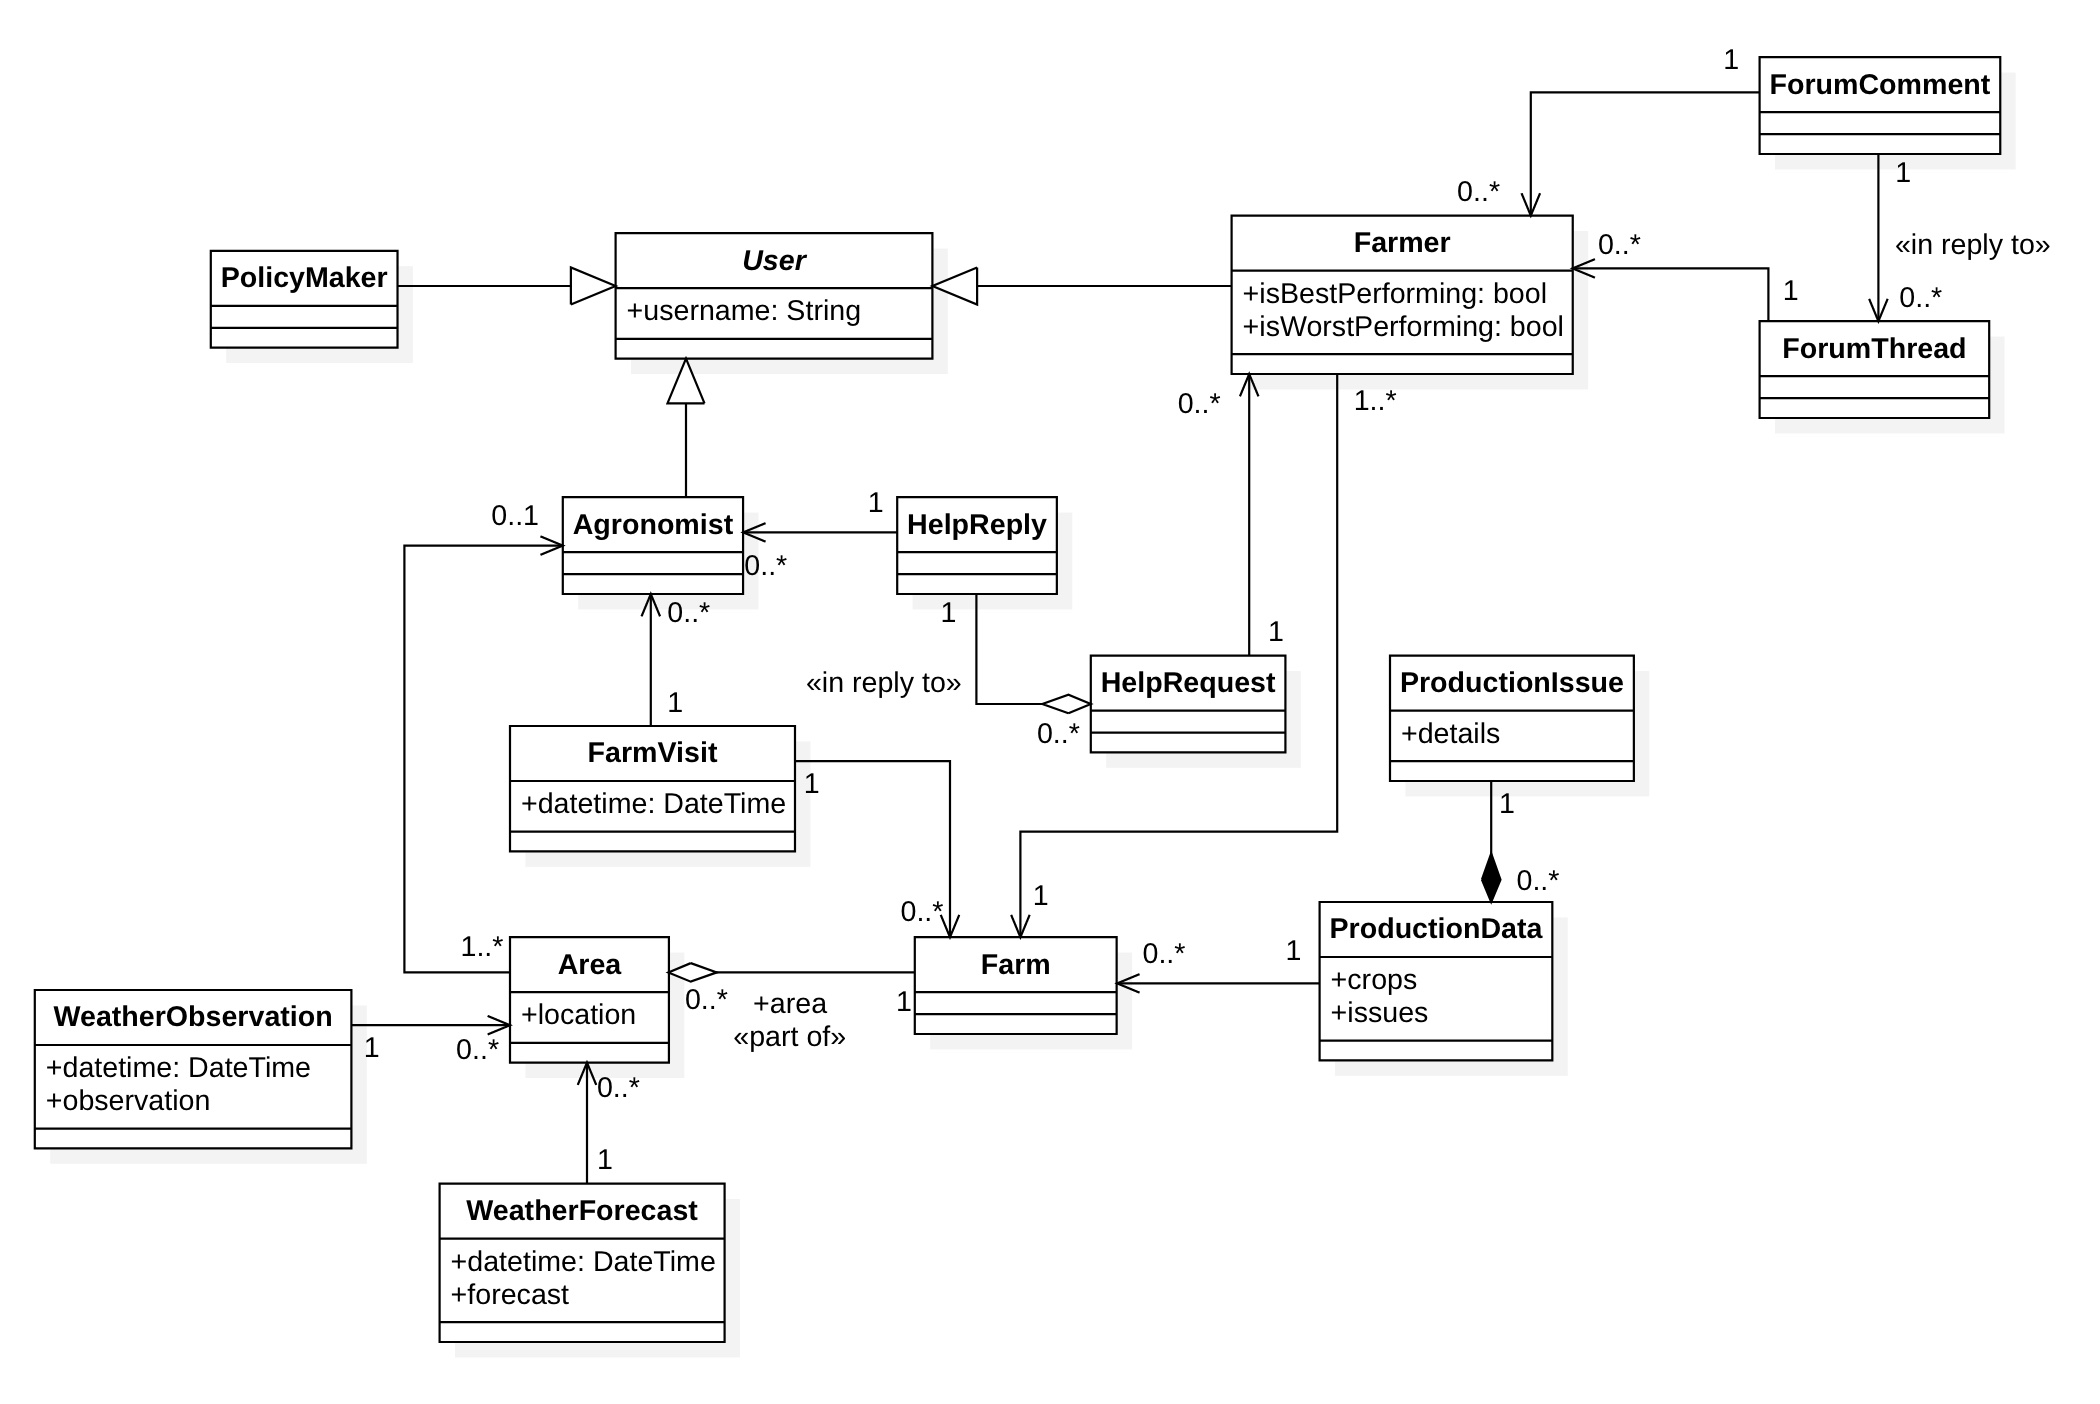
\includegraphics[scale=0.35]{class_diagrams/requirements-level class diagram.png}
    \caption{Requirements-level class diagram of DREAM.}
\end{figure}

The state diagram for the creation of a new help request is:
\begin{figure}[H]
    \centering
	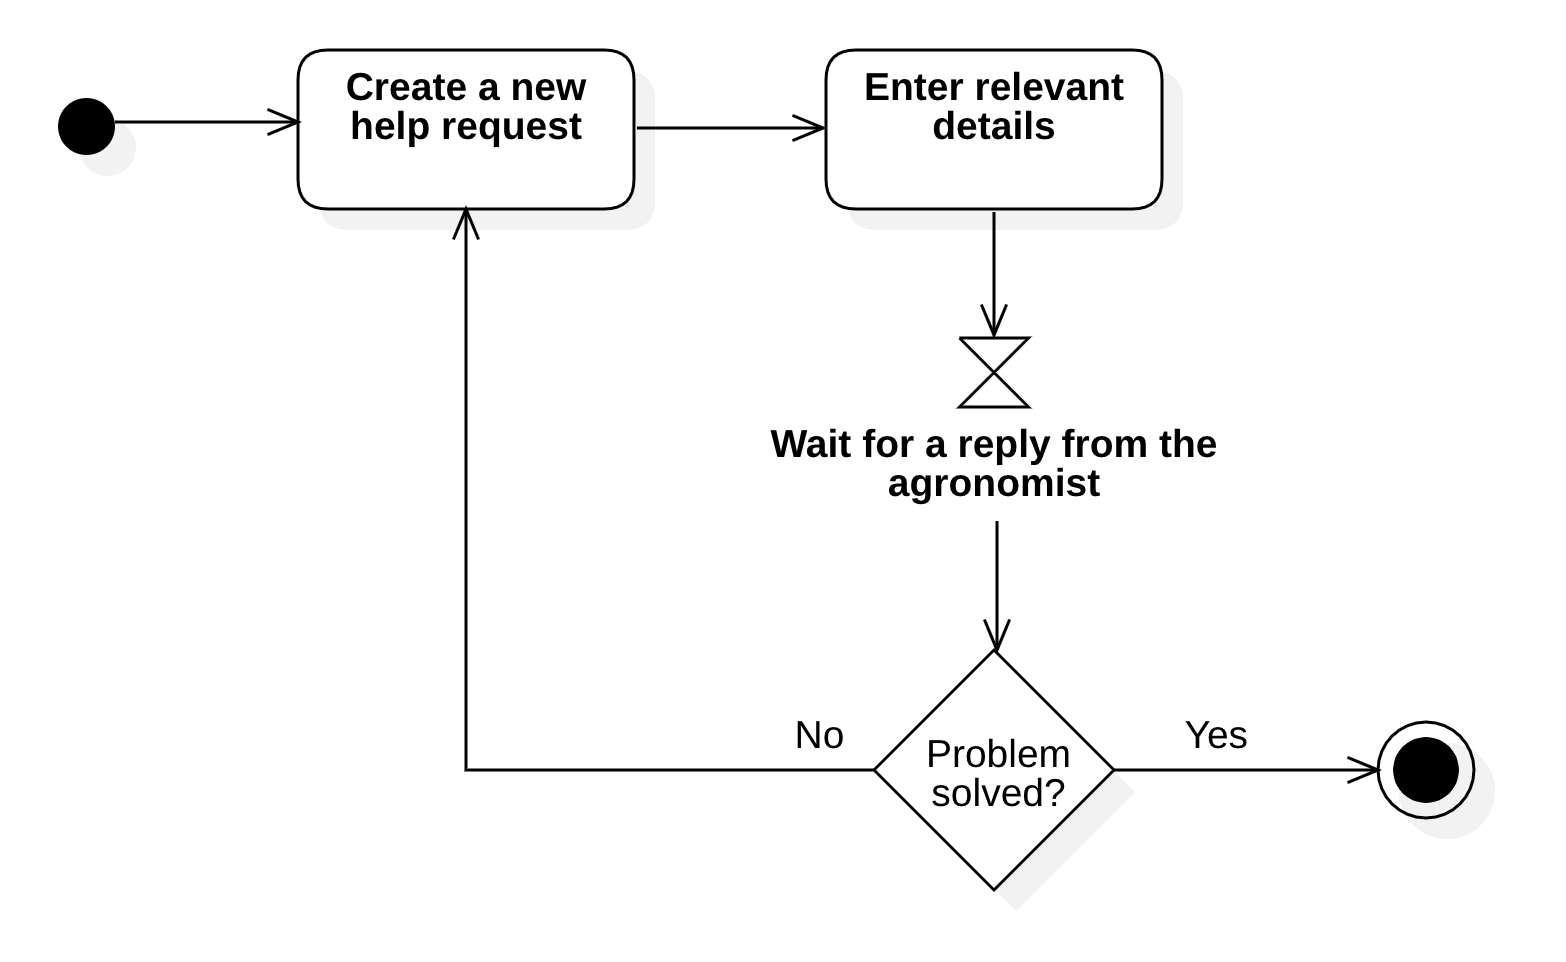
\includegraphics[scale=0.35]{state_machine_diagrams/statediagram1.png}
    \caption{State diagram for the creation of a new help request.}
\end{figure}

The state diagram for the generation of a new daily plan is:
\begin{figure}[H]
    \centering
	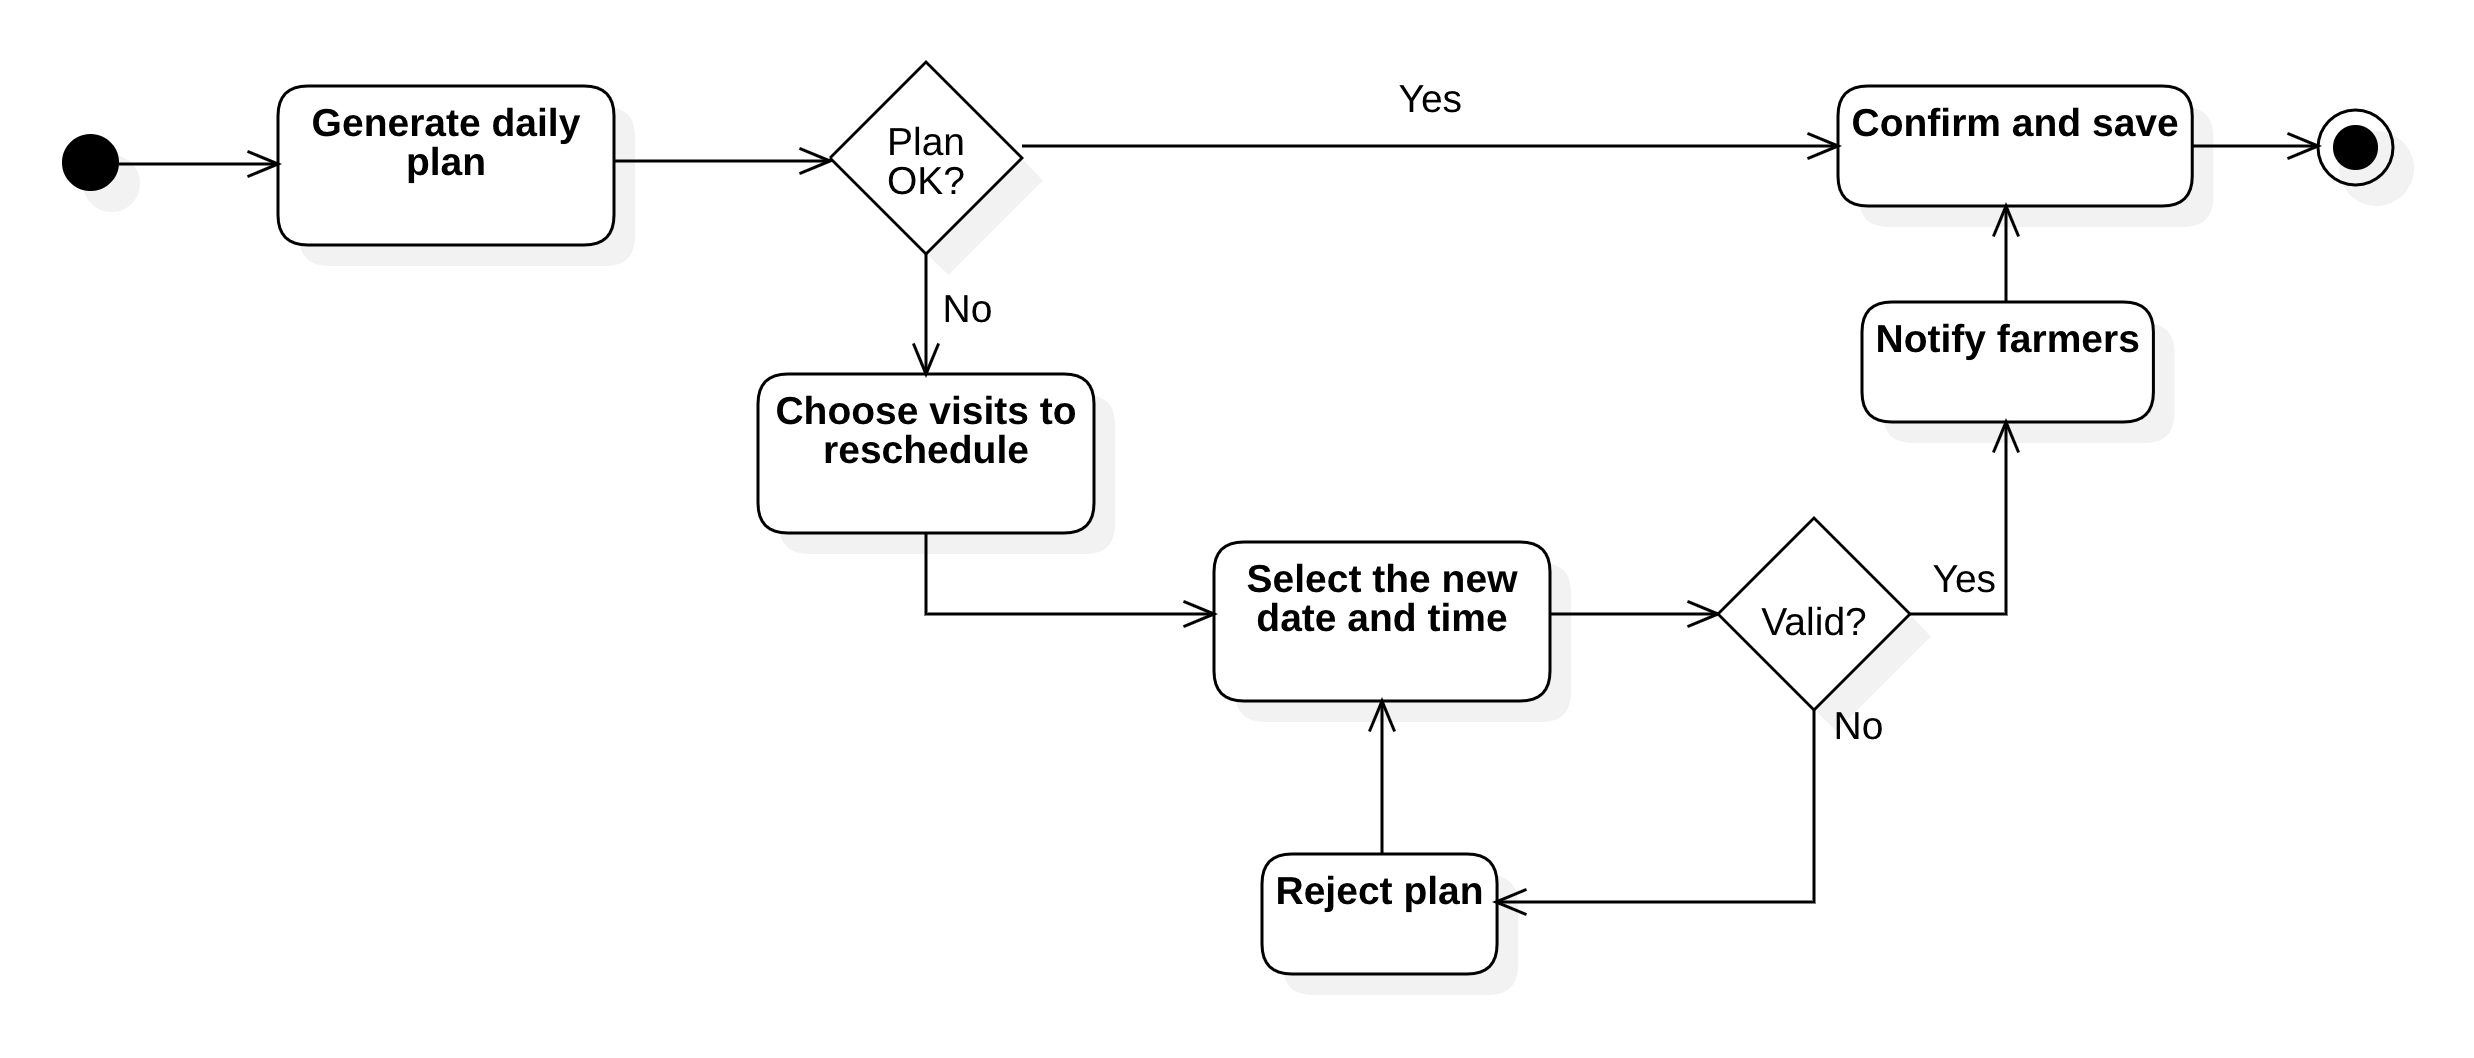
\includegraphics[scale=0.35]{state_machine_diagrams/statediagram2.png}
    \caption{State diagram for the generation of a new daily plan.}
\end{figure}
The state diagram for the creation of a new production report is:
\begin{figure}[H]
    \centering
	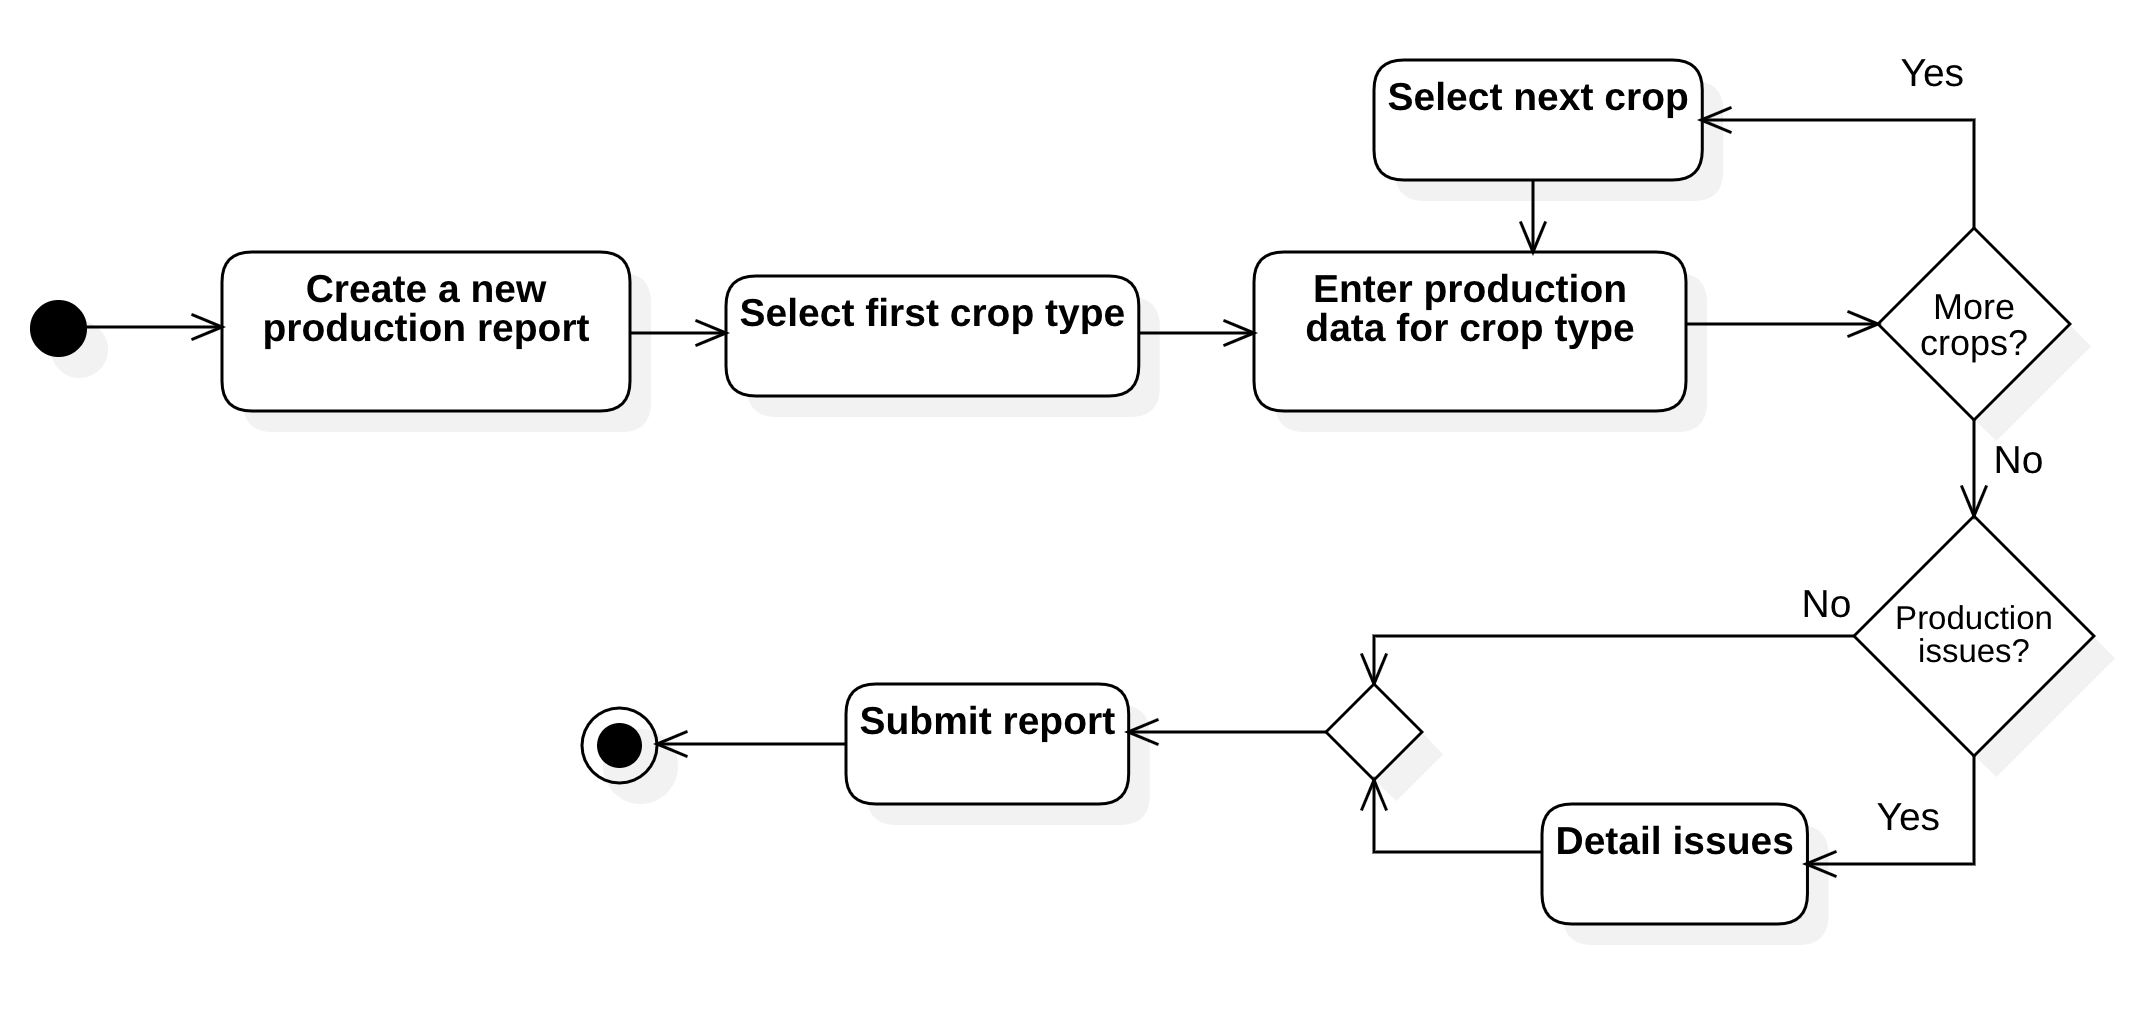
\includegraphics[scale=0.35]{state_machine_diagrams/statediagram3.png}
    \caption{State diagram for the creation of a new production report.}
\end{figure}
\subsection{Product functions} \label{Product functions}
In this section, a list of the most important requirements of the system is provided; notice 
that they are just briefly described, since they will be analysed in-depth in chapter 3.
\subsubsection{Data collection}
Just like every data-driven decision, data is essential. \verb |DREAM| must be able to manage different kinds of data coming from different sources:
\begin{enumerate}
\item agronomists and farmers insert into the system standard kind of information about the farms they 
respectively visit and own, but also other kinds of information like, for example, the types of products 
cultivated and the production volume for each product (kinds of information that allow the analytics to 
profile these users). \verb |DREAM| also allows them to insert less-structured data, for instance full-text feedback 
about the inserted data (farmers can insert data about any problem they face);
\item data gathered by sensors deployed on the territory and by the water irrigation system are automatically 
collected by \verb|DREAM| through effective interfaces interacting with such systems;
\item already existing systems are integrated with \verb|DREAM|;
\item the last but not the least, farmers can interact through discussion forums, that are stored by \verb|DREAM|.
\end{enumerate}
\subsubsection{Data analysis}
The raw data collected by \verb|DREAM| must be processed before being delivered to the end-user. Therefore, 
starting with the big volume of information “ingested”, various kinds of analytics are performed in order to 
provide a more aggregate version of the data:
\begin{itemize}
%machine learning techniques are used to customize (for example) the suggestions recommended to the 
%farmers based on their location and their type of production;
\item the suggestions provided to the farmers are customized according to their information;
\item information about farmers’ production is used to distinguish among farmers who are performing well 
and those who are not;% (classification problem);
%data mining algorithms are used to track patterns and identify relations
\item  patterns and relations are identified among the data (for instance between weather 
forecasts and production volumes);
% statistical algorithms are applied for quantifying the improvement (if present) in the crop after having 
% adopted agronomists’ suggestions.
\item analytics are also used for quantifying the improvement (if present) in the crop after having adopted agronomists’ suggestions.
\end{itemize}
\subsubsection{Forum}
As previously mentioned, farmers are allowed to open discussion forums on \verb|DREAM| with other farmers. 
This allows to keep in touch with other people doing the same job and, hence, to ask for advice in case of 
needing.
\subsubsection{Request and supply of help}
There are 4 different ways for a farmer to ask for help: ask for it directly to other farmers, ask in the forum, ask to to
the agronomists or waiting for the system to recognize him as in trouble. As far as the first option is 
concerned, the service is provided through a GUI. On the other side, either farmers who are performing 
well or agronomists may be reached by the system on behalf of other farmers (or of the system itself) for a 
request of help. Then the system introduces them. It should be remarked that a farmer can contact only 
agronomists in the same area.
\subsubsection{Daily plan}
\verb|DREAM| automatically devises a daily plan for each agronomist consisting in a list of farms that must be visited and provides a possible time schedule for such meetings. Every daily plan must be actively accepted 
by the agronomist before the involved farmer is notified. Anyway, the agronomist can apply some changes 
to the schedule, but the system will not approve them if some constraints are violated.
\subsection{User characteristics}
With regards to the possible actors of \verb|DREAM|, three different main user classes can be identified:
\begin{description}
\item \textbf{Policy makers}: their job is to devise policies to regulate the agricultural production. \verb|DREAM| helps 
them providing aggregate data. Policy makers access the system and then receive high-level 
information about which farmers are performing well and which not, and possible reasons to this 
fact. Furthermore, \verb|DREAM| helps to understand the impact of agronomists’ clues in farmers’ 
productions;
\item \textbf{Farmers}: they have a farm and some plots of land to cultivate. They access the system and insert 
data about themselves, helping \verb|DREAM| to profile them. They insert data about their productions, 
the area where they work, eventual problems they must face, questions in the forum … and so on. 
On the other side, \verb|DREAM| puts them in touch with someone who can help them and provides data 
that may be relevant to them;
\item \textbf{Agronomists}: an agronomist has to find methods for increasing the production and the quality of 
the harvest. They insert the area they are responsible of and the they receive data about the best 
performing farmers and weather forecasts. They can answer to farmers’ questions and they receive 
a raw daily plan about which farmers they should visit.
\end{description}
\subsection{Assumptions, dependencies and constraints}

\rowcolors{2}{gray!15}{gray!35}
\begin{longtable}[c]{|m{0.75cm}|m{11cm}|}
%%%%%%%%%%%%%%%%%%%%%%%%%%%%%%%%%%
 \hline
 \multicolumn{2}{|c|}{\cellcolor{white}\textbf{\emph{Domain assumptions}}}
 % do not write anything here
 \endfirsthead
 % do not write anything here
 \endhead
 % do not write anything here
 \endfoot
 % do not write anything here
 \endlastfoot
%%%%%%%%%%%%%%%%%%%%%%%%%%%%%%%%%
  \hline
  D1 & The location of the sensors is known to the \verb|DREAM| system.\\
  \hline
   D2 & The location of the water irrigation systems is known to the \verb|DREAM| system .\\
  \hline
  D3 & The TSDPS provides weather forecasts and reports which can be accessed by \verb|DREAM|.\\
  \hline
  D4 & The weather reports provide sufficiently accurate data.\\
  \hline
  D5 & The water irrigation system provides data to the DREAM with a sufficiently accurate precision.\\
  \hline
  D6 & Soil moisture sensors provide data with a sufficiently accurate precision.\\
  \hline
  D7 & Each farmer owns at least one device connected to Internet.\\
  \hline
  D8 & Each farmer has the competences for properly accessing the \verb|DREAM| system and registering to it.\\
  \hline
  D9 & All the data the farmers insert is correct.\\
  \hline
  D10 & The farmers answer to help requests when they find one on the system.\\
  \hline
  D11 & When a farmer does something to a certain area (for example, applies a fertilizer or harvests), he covers the whole area.\\
  \hline
  D12 & Each policy maker owns a personal computer, connected to the Internet network and with a browser installed.\\
 \hline
  D13 & Each policy maker has the competences for properly accessing the \verb|DREAM| system and using it.\\
  \hline
  D14 & Every policy maker is given a password – associated to his e-mail – by the Telangana agriculture department, and such account is known to \verb|DREAM|.\\
  \hline
  D15 & Each agronomist owns a device connected to the Internet network and with a browser installed.\\
  \hline
  D16 & The agronomists are given a password – associated to their mail – by the Telangana agriculture department and such account is known to \verb|DREAM|.\\
  \hline
  D17 & Each agronomist has the competences for properly accessing the \verb|DREAM| system and using it.\\
   \hline
  D18 & All the data the agronomists insert is correct.\\
  \hline
  D19 & The agronomists reply to help requests issued by farmers.\\
  \hline
  \end{longtable}
\section{Specific requirements}
\subsection{External Interface Requirements}
\subsubsection{User interfaces}
\verb|DREAM| is provided to the users, namely farmers, agronomists and policy makers, as a webapp, accessible through a browser on the web. Therefore, \verb|DREAM| is not given with a CLI\footnote{Command Line Interface} but only with a GUI\footnote{Graphical User Interface}. The rest of this subsection contains some mockups that show an example of suitable user interface for \verb|DREAM|\footnote{According to the “IEEE 29148-2018 Requirements engineering” document, section 9.6.4.2, “A style guide for the user interface can provide consistent rules for organization, coding and interaction of the user with the system”.}.
\subsubsection{Hardware interfaces}
\begin{itemize}
\item Because \verb|DREAM| is to be implemented as a webapp, every user can access it through the device he prefers, that is personal computers, smartphones, tablets … and the only requirement for the webapp is to be responsive (make the website scale properly to different devices’ sizes). Every device of this kind suffices to achieve the goals.
\item \verb|DREAM| has to interact with various hardware components to gather the data it will use. In particular, \verb|DREAM| has to interact with soil sensors and a water irrigation system. Both these two systems are able to gather data and share it through a third already existing system (an IoT hub), to which they are connected through cables.
\end{itemize}
\subsubsection{Software interfaces}
The following software interfaces are required to make \verb|DREAM| work properly:
\begin{enumerate}
\item every user’s device must have a browser installed on it through which the user can access the \verb|DREAM|’s website; no other software requirements are requested to these kind of devices;
\item \verb|DREAM| requires the APIs to the Telangana’s government website\footnote{\url{https://www.tsdps.telangana.gov.in/aws.jsp}.} in order to retrieve weather reports and meteorological short-term and long-term forecasts;
\item \verb|DREAM| requires also an interface to the system that provides access to the data gathered by soil sensors and by the water irrigation system.
\end{enumerate}
\subsubsection{Communication interfaces}
As far as the communication interfaces are concerned, \verb|DREAM| uses:
\begin{enumerate}
    \item the HTTP protocol at the application layer (layer 7 of the stack) to exchange information (web pages) with the clients (users’ devices) and to access the data offered by the Telangana’s government systems;
    \item specific protocols, such as MQTT\footnote{\url{https://mqtt.org/}.} for communication to the sensor hub.
\end{enumerate}

\subsection{Functional Requirements}
\verb |DREAM| allows its users to perform many tasks, and \verb |DREAM| itself is able to interact with other different systems to achieve some results (see section \ref{Product functions}). In order to provide the main requirements of the system and a summary of the possible situations in which \verb |DREAM| is involved and used, this paragraph first lists all the requirements of the system, then it lists some concrete scenarios \footnote{“A narrative description of what people do and experience as
they try to make use of computer systems and applications” [M.
Carrol, Scenario-based Design, Wiley, 1995]} and finally it abstracts from details and specificities showing the corresponding use cases.
\subsubsection{Requirements}

\rowcolors{2}{gray!15}{gray!35}
\begin{longtable}[c]{|m{0.75cm}|m{11cm}|}
%%%%%%%%%%%%%%%%%%%%%%%%%%%%%%%%%%
 \hline
 \multicolumn{2}{|c|}{\cellcolor{white}\textbf{\emph{Requirements}}}
 % do not write anything here
 \endfirsthead
 % do not write anything here
 \endhead
 % do not write anything here
 \endfoot
 % do not write anything here
 \endlastfoot
%%%%%%%%%%%%%%%%%%%%%%%%%%%%%%%%%
  \hline
  R1\label{R} & \verb|DREAM| collects soil moisture data from the soil moisture sensors;\\
  \hline
  R2\label{R} & \verb|DREAM| accesses weather reports data provided by the TSDPS system;\\
  \hline
  R3\label{R} & \verb|DREAM| collects watering data from the water irrigation system;\\
  \hline
R4\label{R} & \verb|DREAM| shall allow agronomists to insert feedback about the farmers they visited;\\
  \hline
R5\label{R} & \verb|DREAM| shall allow farmers to insert the location and the area of their plot of land;\\
\hline
R6\label{R} & \verb|DREAM| shall allow farmers to insert the type of products they grow in a certain area of their farms;\\
\hline
R7\label{R} & \verb|DREAM| shall allow farmers to insert data about their sowing activity;\\
\hline
R8\label{R} & \verb|DREAM| shall allow farmers to insert data about their planting activity;\\
  \hline
  R9\label{R} & \verb|DREAM| shall allow farmers to insert data about their harvesting activity;\\
  \hline
  R10\label{R} & \verb|DREAM| shall allow farmers to insert data about the irrigation of their plantations;\\
  \hline
  R11\label{R} & \verb|DREAM| shall allow farmers to insert descriptions of problems they face\\
  \hline
R12\label{R} & \verb|DREAM| can use different criteria (namely, productivity in terms of harvested quantity over sowed quantity, productivity in presence of adverse meteorological events, productivity in presence of drought, and so on) and/or combinations of them to rank farmers;\\
  \hline
R13\label{R} & \verb|DREAM| shall allow policy makers to choose the criteria to use for ranking farmers and the associated weights (for combinations of them);\\
  \hline
R14\label{R} & \verb|DREAM| shall allow policy makers to choose the time period and the area to consider for ranking the farmers;\\
  \hline
R15\label{R} & \verb|DREAM| is able to show a list of farmers ordered with respect to the provided ranking criteria\\
  \hline
  R16\label{R} & \verb|DREAM| allows policy makers to mark a farmer as best-performing or worst-performing\\
  \hline
R17\label{R} & \verb|DREAM| can compare different time periods of a farmer work according to various production criteria (e.g. production volume, fertilizers adopted, fraction of harvested plants over sowed ones, etc);\\
  \hline
R18\label{R} & \verb|DREAM| can compare different time periods of a  farmer work with respect to environmental factors (e.g. weather reports data, soil moisture, ...);\\
  \hline
R19\label{R} & \verb|DREAM| allows policy makers to choose an initiative taken by an agronomist or a farmer to help a farmer - i.e., visit to the farm or reply to a question - and two time periods of the farmer to compare the two time periods;\\
  \hline
R20\label{R} & \verb|DREAM| can show the impact of a certain initiative taken by an agronomist or a farmer to help a farmer - i.e., visit to the farm or reply to a question - during a certain time period.\\
  \hline
  R21\label{R} & \verb|DREAM| is able to find correlations among environmental factors, fertilisers adopted and crops planted with the volume of production of the farmers;\\
  \hline
R22\label{R} & \verb|DREAM| allows farmers to choose the date of the forecasts to visualize;\\
  \hline
R23\label{R} & \verb|DREAM| is able to connect to the Telangana government website to fetch forecasts for the chosen date;\\
  \hline
R24\label{R} & \verb|DREAM| can show weather forecast data for a certain location and date.\\
  \hline
R25\label{R} & \verb|DREAM| shall allow agronomists to insert the area they are responsible of;\\
  \hline
R26\label{R} & \verb|DREAM| shall allow agronomists to choose the date of the weather forecasts to visualize;\\
  \hline
R27\label{R} & \verb|DREAM| can make predictions about the crops to plant and fertilizers to use given certain weather forecasts;\\
  \hline
R28\label{R} & \verb|DREAM| allows farmers to choose the (best-performing) farmer or agronomist who to issue a request;\\
  \hline
R29\label{R} & \verb|DREAM| allows the farmers to send a request to a best-performing farmer or agronomist;\\
  \hline
R30\label{R} & \verb|DREAM| notifies (best-performing) farmers and agronomists of the requests of help from other farmers;\\
  \hline
R31\label{R} & \verb|DREAM| allows best-performing farmers and agronomists to insert a message of response to the farmers who have made a request for help to them;\\
  \hline
R32\label{R} & \verb|DREAM| sends the response to the farmer who issued the corresponding request;\\
  \hline
R33\label{R} & \verb|DREAM|EAM allows farmers to initiate a new thread in the forum;\\
  \hline
R34\label{R} & \verb|DREAM|AM allows the farmers to add a post to a thread in the forum;\\
  \hline
R33\label{R} & DREAM allows agronomists to choose the criteria to use for ranking and, potentially, some associated weights (for combinations of them);\\
  \hline
R34\label{R} & DREAM allows agronomists to choose the period and the area to consider for ranking the farmers;\\
  \hline
R35\label{R} & DREAM can show a list of farmers with the corresponding rankings and allow agronomists to mark them as best or worst-performing;\\
  \hline
R36\label{R} & DREAM shall store all the dates of the visits received by a certain farmer, and the agronomist who performed the visit;\\
  \hline
R37\label{R} & DREAM is able to generate a daily plan of visits for each agronomist evenly distributing (with exceptions to bad-performing farmers) over the year the number of visits to each farmer;\\
  \hline
R38\label{R} & DREAM is able to generate a daily plan of visits for each agronomist forcing every farmer to be visited at least twice a year;\\
  \hline
R39\label{R} & DREAM is able to generate a daily plan of visits for each agronomist such that farmers with lower rankings are visited more often than those with higher rankings;\\
  \hline
R40\label{R} & DREAM allows the agronomists to accept or modify the autogenerated daily plan;\\
  \hline
R41\label{R} & DREAM is able to check whether the modifies to a daily plan added by an agronomist are acceptable;\\
  \hline
R42\label{R} & DREAM is able to notify the farmers involved by a visit of an agronomist.\\
  \hline
  \end{longtable}
  \newpage
\subsubsection{Mapping \texorpdfstring{$R \wedge D \vDash G$}{TEXT}}
This section is about showing that the previously listed requirements and domain assumptions can be used to satisfy the goals. In table \ref{rg mapping} you can see a summary of the implications, while in the rest of the section you can find some explanations of such entailments.

\rowcolors{2}{gray!15}{gray!35}
\begin{longtable}[c]{|m{0.15cm}|m{0.15cm}|m{0.15cm}|m{0.15cm}|m{0.15cm}|m{0.15cm}|m{0.15cm}|m{0.15cm}|m{0.15cm}|m{0.15cm}|m{0.15cm}|}
 \caption{Traceability matrix of requirements and domain assumptions to goals.}
 \label{rg mapping}
%%%%%%%%%%%%%%%%%%%%%%%%%%%%%%%%%%
 \hline
 \multicolumn{11}{|c|}{\cellcolor{white}$R \wedge D \vDash G$}
 % do not write anything here
 \endfirsthead
 \hline
  \cellcolor{yellow!30} & \cellcolor{white}G1 & \cellcolor{white}G2 & \cellcolor{white}G3 & \cellcolor{white}G4 & \cellcolor{white}G5 & \cellcolor{white}G6 & \cellcolor{white}G7 & \cellcolor{white}G8 & \cellcolor{white}G9 & \cellcolor{white}G10 \\
 \endhead
 % do not write anything here
 \endfoot
 % do not write anything here
 \endlastfoot
%%%%%%%%%%%%%%%%%%%%%%%%%%%%%%%%%
 \hline
  \cellcolor{yellow!30} & \cellcolor{white}G1 & \cellcolor{white}G2 & \cellcolor{white}G3 & \cellcolor{white}G4 & \cellcolor{white}G5 & \cellcolor{white}G6 & \cellcolor{white}G7 & \cellcolor{white}G8 & \cellcolor{white}G9 & \cellcolor{white}G10 \\
 \hline
 D1 &   &   &   &   &   &   &   &   &   &   \\
 \hline
 D2 &   &   &   &   &   &   &   &   &   &   \\
 \hline
 D3 &   &   &   &   &   &   &   &   &   &   \\
 \hline
 D4 &   &   &   &   &   &   &   &   &   &   \\
 \hline
 D5 &   &   &   &   &   &   &   &   &   &   \\
 \hline
 D6 &   &   &   &   &   &   &   &   &   &   \\
 \hline
 D7 &   &   &   &   &   &   &   &   &   &   \\
 \hline
 D8 &   &   &   &   &   &   &   &   &   &   \\
 \hline
 D9 &   &   &   &   &   &   &   &   &   &   \\
 \hline
 D10 &   &   &   &   &   &   &   &   &   &   \\
 \hline
 D11 &   &   &   &   &   &   &   &   &   &   \\
 \hline
 D12 &   &   &   &   &   &   &   &   &   &   \\
 \hline
 D13 &   &   &   &   &   &   &   &   &   &   \\
 \hline
 D14 &   &   &   &   &   &   &   &   &   &   \\
 \hline
 D15 &   &   &   &   &   &   &   &   &   &   \\
 \hline
 D16 &   &   &   &   &   &   &   &   &   &   \\
 \hline
 D17 &   &   &   &   &   &   &   &   &   &   \\
 \hline
 D18 &   &   &   &   &   &   &   &   &   &   \\
 \hline
 D19 &   &   &   &   &   &   &   &   &   &   \\
 \hline
 R1 & X & X & X &   & X &   & X &   &   & X \\
 \hline
 R2 & X & X & X &   & X &   & X &   &   & X \\
 \hline
 R3 & X & X & X &   & X &   & X &   &   & X \\
 \hline
 R4 & X & X & X & X & X &   & X &   &   & X \\
 \hline
 R5 & X &   &   &   &   &   & X &   &   & X \\
 \hline
 R6 & X &   &   &   &   &   &   &   &   &   \\
 \hline
 R7 & X &   &   &   &   &   &   &   &   &   \\
 \hline
 R8 & X &   &   &   &   &   &   &   &   &   \\
 \hline
 R9 &   & X &   &   &   &   &   &   &   &   \\
 \hline
 R10 &   & X & X &   &   &   &   &   &   &   \\
 \hline
 R11 &   & X & X &   &   &   &   &   &   &   \\
 \hline
 R12 &   & X &   &   &   &   &   &   &   &   \\
 \hline
 R13 &   & X &   &   &   &   &   &   &   &   \\
 \hline
 R14 &   &   & X &   & X &   &   &   &   &   \\
 \hline
 R15 &   &   & X &   &   &   &   &   &   &   \\
 \hline
 R16 &   &   &   & X &   &   &   &   &   &   \\
 \hline
 R17 &   &   &   & X & X &   &   &   & X &   \\
 \hline
 R18 &   &   &   & X &   &   &   &   & X &   \\
 \hline
 R19 &   &   &   &   &   &   & X &   & X &   \\
 \hline
 R20 &   &   &   &   &   &   &   &   & X &   \\
 \hline
 R21 &   &   &   &   & X &   &   &   &   &   \\
 \hline
 R22 &   &   &   &   & X &   &   &   &   &   \\
 \hline
 R23 &   &   &   &   &   & X &   &   &   &   \\
 \hline
 R24 &   &   &   &   &   & X &   &   &   &   \\
 \hline
 R25 &   &   &   &   &   & X &   &   &   &   \\
 \hline
 R26 &   &   &   &   &   & X &   &   &   &   \\
 \hline
 R27 &   &   &   &   &   & X &   &   &   &   \\
 \hline
 R28 &   &   &   &   &   & X &   &   &   &   \\
 \hline
 R29 &   &   &   &   &   &   &   & X &   &   \\
 \hline
 R30 &   &   &   &   &   &   &   & X &   &   \\
 \hline
 R31 &   &   &   &   &   &   &   & X &   &   \\
 \hline
 R32 &   &   &   &   &   &   &   & X &   &   \\
 \hline
 R33 &   &   &   &   &   &   & X &   &   & X \\
 \hline
 R34 &   &   &   &   &   &   & X &   &   & X \\
 \hline
 R35 &   &   &   &   &   &   & X &   &   & X \\
 \hline
 R36 &   &   &   &   &   &   & X &   &   &   \\
 \hline
 R37 &   &   &   &   &   &   & X &   &   &   \\
 \hline
 R38 &   &   &   &   &   &   & X &   &   &   \\
 \hline
 R39 &   &   &   &   &   &   & X &   &   &   \\
 \hline
 R40 &   &   &   &   &   &   & X &   &   &   \\
 \hline
 R41 &   &   &   &   &   &   & X &   &   &   \\
 \hline
 R42 &   &   &   &   &   &   & X &   &   &   \\
 \hline
\end{longtable}
Now an explanation of why a certain goal is entailed by certain requirements and certain domain assumptions is provided.
\vspace{1cm}
\textbf{G1: The policy makers are able to identify the best-performing farmers and the worst-performing farmers.}
\begin{itemize}
    \item R1 \verb|DREAM| collects and accesses data like soil moisture, weather reports (temperature, ...), water used for irrigation with a timestamp and the concerned area;
    \item R2 \verb|DREAM| collects feedbacks of agronomists about farmers and problems faced by farmers with a timestamp and the concerned farmer;

    \item R3 DREAM collects data about farmers, like volume of production, fertilizers adopted, ... with the concerned farmer and the relative period;

    \item R4 DREAM shall store the area of the farm of each farmer;

    \item R5 DREAM can make use of different criteria (namely, which data like soil moisture... use to compare farmers) and/or combinations of them to rank farmers;

    \item R6 DREAM allows policy makers to choose the criteria to use for ranking and, potentially, some associated weights (for combinations of them);

    \item R7 DREAM allows policy makers to choose the period and the area to consider for ranking the farmers;

    \item R8 DREAM can show a list of farmers with the corresponding rankings and allow policy makers to mark them as best or worst-performing.
\end{itemize}
In order to achieve this goal, \verb|DREAM| must be able to collect all the data that may be correlated to the performances of a farmer (R1, R2, R3, R4); moreover, some criteria to assign weights to the various factors have to be chosen (R5, R6, R7). Finally, \verb|DREAM| must be able to show the results to the user (R8).

\vspace{5mm}
\textbf{G2: The policy makers are able to understand whether the initiatives involving agronomists and best-performing farmers have a good impact on the work of the farmers.}
\begin{itemize}
    \item R1 DREAM collects and accesses data like soil moisture, weather reports (temperature, ...), water used for irrigation with a timestamp and the concerned area;

    \item R2 DREAM collects feedbacks of agronomists about farmers and problems faced by farmers with a timestamp and the concerned farmer;

    \item R3 DREAM collects data about farmers, like volume of production, fertilizers adopted, ... with the concerned farmer and the relative period;

    \item R4 DREAM shall store the area of the farm of each farmer;

    \item R9 DREAM shall store the initiatives involving agronomists and best-performing farmers currently adopted, along with the farmers and agronomists involved and the period of the initiative;

    \item R10 DREAM can compare different periods of farmers work according to the production volume, the fertilizers adopted, ...;

    \item R11 DREAM can compare different periods of farmers work according to environmental factors (e.g. data in weather reports, soil moisture, ...);

    \item R12 DREAM allows policy makers to choose the old period to compare with, and according to which initiative decision;

    \item R13 DREAM can show the impact of a certain initiative during a certain period.
\end{itemize}
Goal G2 is achieved by forcing \verb|DREAM| to collect all the data that may be involved in correlations between initiatives and impact on work (R1, R2, R3, R4, R9); furthermore, \verb|DREAM| must be able to compare different periods of farmers work (R10, R11) according to the choice of the policy maker (R12) and to show the results (R13).

\vspace{5mm}
\textbf{G3 The policy makers receive high-level reports about the impact of some environmental factors and the volume of production of the farmers.}
\begin{itemize}
    \item R1 DREAM collects and accesses data like soil moisture, weather reports (temperature, ...), water used for irrigation with a timestamp and the concerned area;

    \item R2 DREAM collects feedbacks of agronomists about farmers and problems faced by farmers with a timestamp and the concerned farmer;

    \item R3 DREAM collects data about farmers, like volume of production, fertilizers adopted, ... with the concerned farmer and the relative period;

    \item R4 DREAM shall store the area of the farm of each farmer;

    \item R10 DREAM can compare different periods of farmers work according to the production volume, the fertilizers adopted, ...;

    \item R11 DREAM can compare different periods of farmers work according to environmental factors (e.g. data in weather reports, soil moisture, ...);

    \item R14 DREAM can apply some machine learning techniques to understand the correlation among environmental factors, fertilisers adopted and crops planted with the volume of production of the farmers;

    \item R15 DREAM can show reports about the correlation among environmental factors and the volume of production of the farmers.
\end{itemize}
This goal is reached by making \verb|DREAM| able to apply data analisys techniques (R14) to the relevant data (R1, R2, R3, R4); such data must be compared by the system (R10, R11) and the results must be shown (R15).

\vspace{5mm}
\textbf{G4 The farmers visualize weather forecasts regarding their piece of land.}
\begin{itemize}
    \item R4 DREAM shall store the area of the farm of each farmer;

    \item R16 \verb|DREAM| allows farmers to choose the date of the forecasts to visualize;

    \item R17 \verb|DREAM| is able to connect to the Telengana government website to fetch forecasts for the chosen date;

    \item R18 DREAM can show a map with the forecast.
\end{itemize}
In order to achieve this goal, \verb|DREAM| must fetch the forecasts (R17) according to the area of the farmer (R4) and the selected date (R16) and it must be able to show the results (R18).

\vspace{5mm}
\textbf{G5 The farmers receive personalized suggestions about crops to plant and fertilizers to use.}
\begin{itemize}
    \item R1 \verb|DREAM| collects and accesses data like soil moisture, weather reports (temperature, ...), water used for irrigation with a timestamp and the concerned area;

    \item R2 \verb|DREAM| collects feedbacks of agronomists about farmers and problems faced by farmers with a timestamp and the concerned farmer;

    \item R3 DREAM collects data about farmers, like volume of production, fertilizers adopted, ... with the concerned farmer and the relative period;

    \item R4 DREAM shall store the area of the farm of each farmer;

    \item R17 \verb|DREAM| is able to connect to the Telengana government website to fetch forecasts for the chosen date;

    \item R14 DREAM can apply some machine learning techniques to understand the correlation among environmental factors, fertilisers adopted and crops planted with the volume of production of the farmers;

    \item R21 DREAM can use the trained machine learning algorithms to make predictions about the crops to plant and fertilizers to use given certain weather forecasts;

    \item R22 DREAM can show the results of predictions about crops to plant and fertilizers to use to the farmers.

    \item \color{red}(what about agronomists' suggestions?).
\end{itemize}
Goal G5 requires that all the relevant data is known to \verb|DREAM| (R1, R2, R3, R4), that \verb|DREAM| is able to retrieve weather forecasts (R17) and that \verb|DREAM| is able to train some algorithms using past data (R14) in order to make predictions for the future (R21). Of course the system must be able to show the results (R22).

\vspace{5mm}
\textbf{G6 The farmers ask for and receive help from agronomists and other farmers.}
\begin{itemize}
    \item R23 DREAM allows the farmers to choose whether asking for help to an agronomists or to other farmers;

    \item R24 DREAM allows the farmers to insert the a request for help with a justification;

    \item R25 DREAM notifies other farmers/agronomists of the requests of help from other farmers;

    \item R26 DREAM allows other farmers/agronomists to insert a message of response to the farmers who have made a request for help;

    \item R27 DREAM sends responses of help to the farmers who asked for help;

    \item R28 DREAM deletes notifications of requests for help when a response has been received.
\end{itemize}
The system must be able to establish a connection among those who ask for help and those who can answer (R23, R24, R25, R26, R27). When a request has been satisfied, the request cannot be answered anymore (R28).

\vspace{5mm}
\textbf{G7 The agronomists can plan farm visits based on the farmers performances.}
\begin{itemize}
    \item R19 DREAM shall store the area each agronomist is responsible of;

    \item R1 \verb|DREAM| collects and accesses data like soil moisture, weather reports (temperature, ...), water used for irrigation with a timestamp and the concerned area;

    \item R2 \verb|DREAM| collects feedbacks of agronomists about farmers and problems faced by farmers with a timestamp and the concerned farmer;

    \item R3 DREAM collects data about farmers, like volume of production, fertilizers adopted, ... with the concerned farmer and the relative period;

    \item R4 DREAM shall store the area of the farm of each farmer;

    \item R5 DREAM can make use of different criteria (namely, which data like soil moisture... use to compare farmers) and/or combinations of them to rank farmers;

    \item R33 DREAM allows agronomists to choose the criteria to use for ranking and, potentially, some associated weights (for combinations of them);

    \item R34 DREAM allows agronomists to choose the period and the area to consider for ranking the farmers;

    \item R35 DREAM can show a list of farmers with the corresponding rankings and allow agronomists to mark them as best or worst-performing;

    \item R36 DREAM shall store all the dates of the visits received by a certain farmer, and the agronomist who performed the visit;

\item R37 DREAM is able to generate a daily plan of visits for each agronomist evenly distributing (with exceptions to bad-performing farmers) over the year the number of visits to each farmer;

\item R38 DREAM is able to generate a daily plan of visits for each agronomist forcing every farmer to be visited at least twice a year;

\item R39 DREAM is able to generate a daily plan of visits for each agronomist such that farmers with lower rankings are visited more often than those with higher rankings;

\item R40 DREAM allows the agronomists to accept or modify the autogenerated daily plan;

\item R41 DREAM is able to check whether the modifies to a daily plan added by an agronomist are acceptable;

\item R42 DREAM is able to notify the farmers involved by a visit of an agronomist.
\end{itemize}
In order to achieve this goal, \verb|DREAM| must be able to rank the various farmers (all the requirements of G10, namely R1, R2, R3, R5, R33, R34, R35) of the area of the agronomist (R4, R19) and remember how many times every farmer has been visited (R36). Then, \verb|DREAM| is required to be able to generate a proposal of daily plan (R37, R38, R39) which can be modified or accepted by the agronomist (R40, R41). Finally, \verb|DREAM| must be able to notify the involved farmer of the meeting (R42).

\vspace{5mm}
\textbf{G8 The farmers can interact with other farmers exchanging opinions about agriculture.}
\begin{itemize}
    \item R29 DREAM allows the farmers to initiate a new thread in the forum;

    \item R30 DREAM allows the farmers to add an answer to a thread in the forum;

    \item R31 DREAM allows the farmers to close threads in the forum;

    \item R32 DREAM allows a farmer to initiate a private chat to another farmer found in the forum.
\end{itemize}
To achieve goal G8, \verb|DREAM| is required to put in contact different farmers through a forum (R29, R30, R31) and, potentially, through a private chat (R32).

\vspace{5mm}
\textbf{G9 The agronomists visualize weather forecasts regarding the area they are responsible of.}
\begin{itemize}
    \item R19 DREAM shall store the area each agronomist is responsible of;

    \item R20 \verb|DREAM| allows agronomists to choose the date of the forecasts to visualize;

    \item R17 \verb|DREAM| is able to connect to the Telengana government website to fetch forecasts for the chosen date;

    \item R18 DREAM can show a map with the forecast.
\end{itemize}
Goal G9 imposes that \verb|DREAM| is able to fetch weather forecasts (R17) according to the area of an agronomist (R19) and the date he has chosen (R20). Of course it shall be able to show the results (R18).

\vspace{5mm}
\textbf{G10 The agronomists are able to identify the best-performing farmers and the worst-performing farmers.}
\begin{itemize}
    \item R1 \verb|DREAM| collects and accesses data like soil moisture, weather reports (temperature, ...), water used for irrigation with a timestamp and the concerned area;

    \item R2 \verb|DREAM| collects feedbacks of agronomists about farmers and problems faced by farmers with a timestamp and the concerned farmer;

    \item R3 DREAM collects data about farmers, like volume of production, fertilizers adopted, ... with the concerned farmer and the relative period;

    \item R4 DREAM shall store the area of the farm of each farmer;

    \item R5 DREAM can make use of different criteria (namely, which data like soil moisture... use to compare farmers) and/or combinations of them to rank farmers;

    \item R33 DREAM allows agronomists to choose the criteria to use for ranking and, potentially, some associated weights (for combinations of them);

    \item R34 DREAM allows agronomists to choose the period and the area to consider for ranking the farmers;

    \item R35 DREAM can show a list of farmers with the corresponding rankings and allow agronomists to mark them as best or worst-performing.
\end{itemize}
This goal forces the system to own all the relevant data for the analysis (R1, R2, R3, R4) and to be able to compare such data (R5) according to choices of the agronomists (R33, R34). Finally, \verb|DREAM| shall be able to show the results.
\subsubsection{Scenarios}
\paragraph{A storm ruined the harvest}
Arin is a farmer who mainly cultivates potatoes, onions and tomatoes in the fields of his family. The harvest of March was really good, and Arin hoped that the same volume of production might have been repeated in April as well. Unfortunately, the North Indian Ocean cyclone season starts in April, and in the second week of this month Tauktae storm, the strongest storm of of the season, violently hit Arin's lands, halving the crop.\par
\noindent Consequently, Arin wants to share in the system (\verb|DREAM|) the outcome of the storm. Arin opens its browser and access the system using its credentials. Next, he selects from a menu in the incoming webpage the entry for inserting data about production and problems. Then he fills the form with a description about the storm and what it caused to its fields, and finally he sends it.\par
\noindent Arin hopes to receive some aid.
\paragraph{Great year for the potatoes}
Like many other farmers in India, Ikbal knows that the best period for cultivating potatoes is during the months from October to December. The weather is neither hot nor cold and the monsoons are nearly over at this time. Therefore, last October Ikbal planted many potatoes, and in February, with the help of some peasants who work for him, has picked up all of them. \par
\noindent In order to publish in \verb|DREAM| the results of this year potatoes' harvest, he access the system through its computer, opens the form for inserting data about the production and then starts to fill it. The form is quite structured, and requires some data for each entry. After having inserted all the objective information about the crop, Ikbal would like to share something he has found out during this year, namely that planting the potatoes at depth x allows to retrieve substantial crops of this vegetable. Thus, Ikbal fills in also the optional text box and then sends it.
\paragraph{Registering to the system as an agronomist}
Dalbir worked for many years as an agronomist in Bihar, but recently he has been moved to Telengana. Telengana uses this innovative system, \verb|DREAM|, to keep track of the harvests of farmers, to collect interesting data from sensors and many other things. All the agronomists in Telengana must work with \verb|DREAM|, therefore Dalbir has to create an account. \par
\noindent Dalbir opens the webpage of \verb|DREAM| and initiates the procedure for creating a new account. He follows the procedure tailored for agronomists, which allows him to create a new username and password. Next, Dalbir has to insert some data about his job in order to finish the registration. Among the others, Dalbir is asked to insert the area where he works.\par
\noindent His data will be verified later.
\paragraph{Visiting a farm}
The first task of Dalbir is to visit the farm of Arin. The date and hour of the meeting has been established by \verb |DREAM|, which has notified also Arin about the meeting. Arin has been chosen because last month he performed very bad.\par
\noindent During the meeting, Arin has the opportunity of explaining all the problems he faced during the past month, one for all Tauktae (the strongest storm of the North Indian Ocean cyclone season). Arin takes Dalbir to the fields, where Dalbir can gather some sample from the terrain. At the end of the meeting, Dalbir gives Arin some advices, and then he moves to another farm. \par
\noindent Once in the office, Dalbir inserts in the system a report about his visit to Arin's farm.
\paragraph{A bad schedule}
Like every evening, Dalbir accesses \verb|DREAM| for downloading the daily plan of the next day. Every daily plan provided by the system contains time and place of every meeting, in addition to some information about the farmer. Dalbir notices that Ikbal's farm is closer to his parents' house, and Dalbir knows that they would be really happy to if he had lunch with them.\par
\noindent However, the meeting with Ikbal is scheduled for the 3p.m o' clock. Therefore, Dalbir decides to exchange the meetings with Ikbal and Tarak, visiting Ikbal at 11.30a.m. and Tarak at 3p.m.. Through the user interface of \verb|DREAM|, Dalbir exhanges the two meetings and once he has confirmed, \verb|DREAM| notifies the farmers of the change.
%\paragraph{Collecting data(?)}
% \verb|DREAM| is a software system designed to provide various kinds of analytics to its users, in particular to the policy makers. As a matter of fact, policy makers want to distinguish between well- and bad- performing farmers, as well as understand the impact of initiatives carried out by the agronomists and find patterns and relations among the data.\par
\noindent Therefore, periodically, \verb|DREAM| interacts with sensors deployed on the territory in order to retrieve the humidity of the soil, with the water irrigation system to retrieve the amount of water used by each farmer and with an already existing website which provides up-to-date weather forecasts. In particular:
\begin{itemize}
    \item 3 times a day the soil sensors are asked to provide data about the humidity of the soil;
    \item once a day the water irrigation system is asked to provide the water used by each farmer (when the data is available);
    \item the weather forecasts website is accessed monthly to compute some analytics on the data, but also on demand when agronomists or farmers ask for weather forecasts.
\end{itemize}

\subsubsection{Use cases}
%\paragraph{Use case 1 - InsertProblems}
%\begin{center} %leave it to start the table at newline

\rowcolors{2}{blue!15}{blue!25}
\begin{longtable}{|p{3.5cm}|m{8cm}|}
 \hline
 \multicolumn{2}{|c|}{\cellcolor{white}\emph{USE CASE 1}} \\
 % do not write anything here
 \endfirsthead
 % do not write anything here
 \endhead
 % do not write anything here
 \endfoot
 % do not write anything here
 \endlastfoot
 \hline
 Name & InsertProblems\\
 \hline
 Actor & Farmer\\
 \hline
 Entry condition & The farmer faces a problem and decides to communicate it on \verb|DREAM|\\
 \hline
 Event flow & \begin{enumerate}
    \item The farmer accesses the system through its username and password;
    \item in the homepage, the farmer selects from the menu the item "insert problem";
    \item the farmer selects the kind of problem, when it occurred and how much it lasted;
    \item the farmer gives a brief description of the problem;
    \item the farmer selects whether he likes to meet as soon as possible an agronomist;
    \item the farmer clicks on the "send" button;
    \item \verb|DREAM| automatically detects where is the farm from the account of the farmer;
    \item \verb|DREAM| stores the data and eventually takes into account the request of a meeting with an agronomist.
 \end{enumerate}\\
 \hline
 Exit condition & The problem is saved in the \verb|DREAM| database and, if requested, an agronomist is scheduled to meet the farmer in the next days. The farmer is notified about the meeting.\\
 \hline
 Exceptions & \begin{itemize}
     \item If the kind of problem is not present, the farmer can add it by its own.
     \item In case no agronomist can be scheduled for the current week, the farmer is notified about the problem and an agronomist will be found for the next week.
 \end{itemize}\\
 \hline
 Special requirements & \begin{itemize}
     \item The availability of an agronomist is checked in less than 3 second;
     \item the page is refreshed in less than 1 second.
 \end{itemize}\\
 \hline
\end{longtable}
\begin{figure}[H]
    \centering
    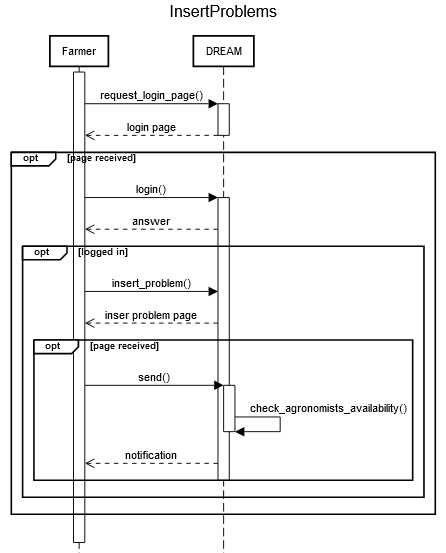
\includegraphics[scale=0.75]{sequence_diagrams/InsertProblems}
    \caption{Sequence diagram for the InsertProblems use case}
\end{figure}
%%%%%%%%%%%TABLE 2%%%%%%%%%%%%%%%%%%%%%%%%%%%%%%%%%%%%%%%%

\centering
\begin{longtable}{|p{3.5cm}|m{8cm}|}
 \hline
 \multicolumn{2}{|c|}{\cellcolor{white}\emph{USE CASE 2}} \\
  % do not write anything here
 \endfirsthead
 % do not write anything here
 \endhead
 % do not write anything here
 \endfoot
 % do not write anything here
 \endlastfoot
 \hline
 Name & InsertProductions\\
 \hline
 Actor & Farmer\\
 \hline
 Entry condition & The farmer gets the results of a crop\\
 \hline
 Event flow & \begin{enumerate}
    \item The farmer accesses the system through its username and password;
    \item in the homepage, the farmer selects from the menu the item "insert productions";
    \item the farmer inserts the picked product, when it was planted, the volume planted, the volume picked;
    \item the farmer optionally gives a brief description of the harvest or an observation he made;
    \item the farmer clicks on the "send" button;
    \item \verb|DREAM| automatically detects where is the farm from the account of the farmer;
    \item \verb|DREAM| stores the data.
 \end{enumerate}\\
 \hline
 Exit condition & The data is saved in the \verb|DREAM| database and the farmer is notified.\\
 \hline
 Exceptions & \begin{itemize}
     \item If the kind of product is not present, the farmer can add it by its own.
 \end{itemize}\\
 \hline
 Special requirements & \begin{itemize}
     \item the page is refreshed in less than 1 second.
 \end{itemize}\\
 \hline
\end{longtable}

\begin{figure}[H]
    \centering
    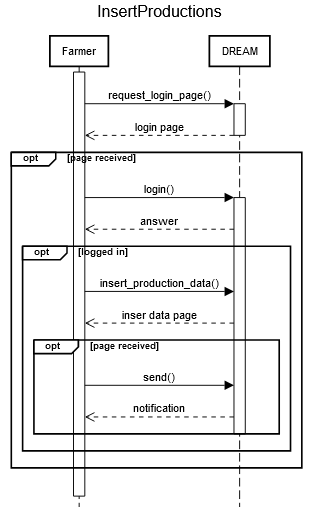
\includegraphics[scale=0.75]{sequence_diagrams/InsertProductions}
    \caption{Sequence diagram for the InsertProductions use case}
\end{figure}
%%%%%%%%%%%%%%%%%%%%%%%%%%%%TABLE 3%%%%%%%%%%%%%%%%%%%%%%%

\centering
\begin{longtable}{|p{3.5cm}|m{8cm}|}
 \hline
 \multicolumn{2}{|c|}{\cellcolor{white}\emph{USE CASE 3}} \\
  % do not write anything here
 \endfirsthead
 % do not write anything here
 \endhead
 % do not write anything here
 \endfoot
 % do not write anything here
 \endlastfoot
 \hline
 Name & RegisterAgronomist\\
 \hline
 Actor & Agronomist\\
 \hline
 Entry condition & The agronomist does not have an account.\\
 \hline
 Event flow & \begin{enumerate}
    \item The agronomist goes to the \verb|DREAM| homepage;
    \item the agronomist selects "create account", then "create agronomist account";
    \item the agronomist inserts his e-mail and devises a password;
    \item the system verifies the e-mail of the agronomist;
    \item the agronomist inserts personal data like name, surname, date of birth, specialization;
    \item the agronomist selects the area where he will work;
    \item the agronomist clicks on "done";
    \item \verb|DREAM| verifies the identity of the agronomist;
    \item the agronomist is notified that he can begin to work.
 \end{enumerate}\\
 \hline
 Exit condition & The agronomist's account is saved in the \verb|DREAM| database and the identity of the agronomist has been verified.\\
 \hline
 Exceptions & \begin{itemize}
     \item If the e-mail is already used, the agronomist is forced to change it;
     \item If the password is too short, the agronomist is forced to change it;
     \item if the identity of the agronomist cannot be verified, a mail notifying the error is sent to the agronomist.
 \end{itemize}\\
 \hline
 Special requirements & \begin{itemize}
     \item the identity must be verified within 3 days.
 \end{itemize}\\
 \hline
\end{longtable}

\begin{figure}[H]
    \centering
    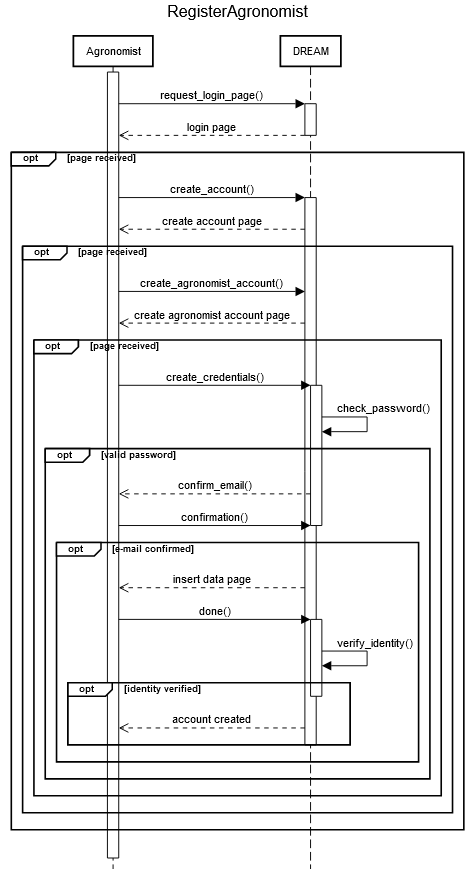
\includegraphics[scale=0.60]{sequence_diagrams/RegisterAgronomist}
    \caption{Sequence diagram for the RegisterAgronomist use case}
\end{figure}
%%%%%%%%%%%%%%%%%%%%%%%%%%%%TABLE 4%%%%%%%%%%%%%%%%%%%%%%%

\centering
\begin{longtable}{|p{3.5cm}|m{8cm}|}
 \hline
 \multicolumn{2}{|c|}{\cellcolor{white}\emph{USE CASE 4}} \\
  % do not write anything here
 \endfirsthead
 % do not write anything here
 \endhead
 % do not write anything here
 \endfoot
 % do not write anything here
 \endlastfoot
 \hline
 Name & RegisterFarmer\\
 \hline
 Actor & Farmer\\
 \hline
 Entry condition & The farmer does not have an account.\\
 \hline
 Event flow & \begin{enumerate}
    \item The farmer goes to the \verb|DREAM| homepage;
    \item the farmer selects "create account", then "create farmer account";
    \item the farmer inserts his e-mail and devises a password;
    \item the system verifies the e-mail of the farmer;
    \item the farmer inserts personal data like name, surname, date of birth, location of the farm;
    \item the farmer clicks on "done";
    \item the farmer is notified that the account has been created.
 \end{enumerate}\\
 \hline
 Exit condition & The farmer's account is saved in the \verb|DREAM| database and the existence of the farm has been verified.\\
 \hline
 Exceptions & \begin{itemize}
     \item If the e-mail is already used, the farmer is forced to change it;
     \item If the password is too short, the farmer is forced to change it.
 \end{itemize}\\
 \hline
 Special requirements &  \\
 \hline
\end{longtable}

\begin{figure}[H]
    \centering
    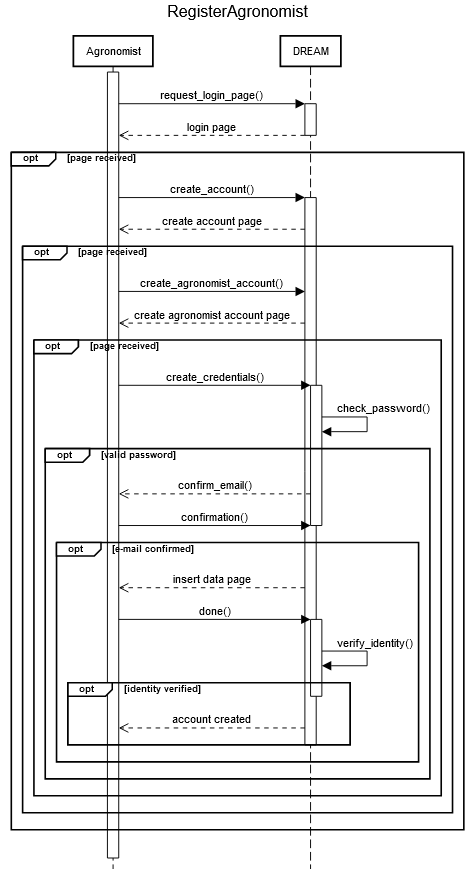
\includegraphics[scale=0.60]{sequence_diagrams/RegisterAgronomist}
    \caption{Sequence diagram for the RegisterFarmer use case}
\end{figure}



%%%%%%%%%%%%%%%%%%%%%%%%%%%%TABLE 5%%%%%%%%%%%%%%%%%%%%%%%

\centering
\begin{longtable}{|p{3.5cm}|m{8cm}|}
 \hline
 \multicolumn{2}{|c|}{\cellcolor{white}\emph{USE CASE 5}} \\
  % do not write anything here
 \endfirsthead
 % do not write anything here
 \endhead
 % do not write anything here
 \endfoot
 % do not write anything here
 \endlastfoot
 \hline
 Name & VisitFarm\\
 \hline
 Actor & Agronomist, Farmer\\
 \hline
 Entry condition & The agronomist is scheduled to visit a farm. The farmer and the agronomist have been informed of the meeting. The time of the meeting occurs.\\
 \hline
 Event flow & \begin{enumerate}
    \item The agronomist is scheduled to visit a certain farm at a certain time;
    \item the farmer is notified about the meeting;
    \item the agronomist accesses \verb|DREAM|;
    \item the agronomist selects "insert farm data";
    \item the agronomist selects the farm and inserts data with a comment;
    \item the agronomist clicks on "done";
    \item \verb|DREAM| stores the data.
 \end{enumerate}\\
 \hline
 Exit condition & The data about the meeting has been inserted by the agronomist and stored in \verb|DREAM|.
 \hline
 Exceptions & \begin{itemize}
     \item If the farmer does not show up at the meeting, the agronomist specifies so when inserting data about the meeting.
 \end{itemize}\\
 \hline
 Special requirements & None\\
 \hline
\end{longtable}


\begin{figure}[H]
    \centering
    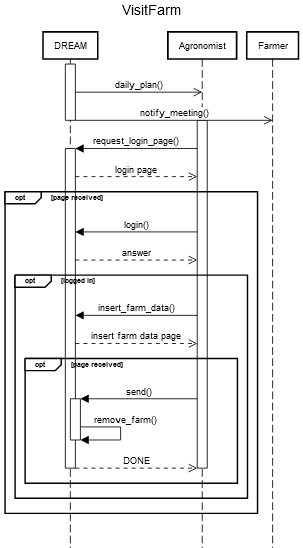
\includegraphics[scale=0.75]{sequence_diagrams/VisitFarm}
    \caption{Sequence diagram for the VisitFarm use case}
\end{figure}
%%%%%%%%%%%%%%%%%%%%%%%%%%%%TABLE 6%%%%%%%%%%%%%%%%%%%%%%%

\centering
\begin{longtable}{|p{3.5cm}|m{8cm}|}
 \hline
 \multicolumn{2}{|c|}{\cellcolor{white}\emph{USE CASE 6}} \\
  % do not write anything here
 \endfirsthead
 % do not write anything here
 \endhead
 % do not write anything here
 \endfoot
 % do not write anything here
 \endlastfoot
 \hline
 Name & GenerateDailyPlan\\
 \hline
 Actor & Agronomist, Farmer\\
 \hline
 Entry condition & The next day is a working day and the agronomist accesses the system.\\
 \hline
 Event flow & \begin{enumerate}
    \item The agronomist receives a daily plan for the following day;
    \item if it is ok for the agronomist, he clicks on  "accept", otherwise he clicks on "change it";
    \item the agronomist selects some changes, then he clicks on "accept";
    \item \verb|DREAM| checks if the new daily plan is acceptable;
    \item the farmer is notified about the meeting.
 \end{enumerate}\\
 \hline
 Exit condition & The daily plan has been confirmed and the farmer has been notified.\\
 \hline
 Exceptions & \begin{itemize}
     \item In case the agronomist does not accept the daily plan, the farmers are not notified about the meeting;
     \item if the daily plan is not acceptable, an error is notified to the agronomist, who has to re-accept (or re-change) the schedule until \verb|DREAM| accepts it;
 \end{itemize}\\
 \hline
 Special requirements &\begin{itemize}
     \item Every farmer must be visited at least twice a year;
     \item bad performing farmers must be visited more times than the others.
 \end{itemize}\\
 \hline
\end{longtable}
\begin{figure}[H]
    \centering
    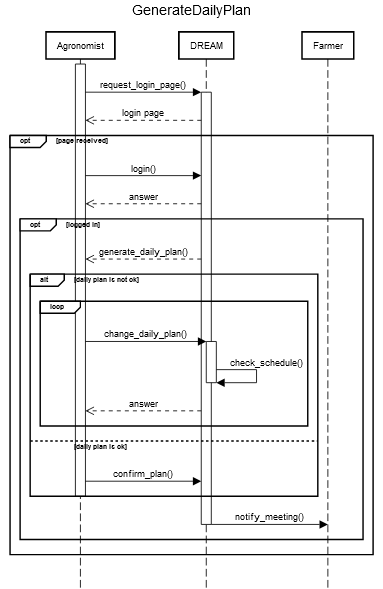
\includegraphics[scale=0.75]{sequence_diagrams/GenerateDailyPlan}
    \caption{Sequence diagram for the GenerateDailyPlan use case}
\end{figure}


%%%%%%%%%%%%%%%%%%%%%%%%%%%%TABLE 7%%%%%%%%%%%%%%%%%%%%%%%

\centering
\begin{longtable}{|p{3.5cm}|m{8cm}|}
 \hline
 \multicolumn{2}{|c|}{\cellcolor{white}\emph{USE CASE 7}} \\
  % do not write anything here
 \endfirsthead
 % do not write anything here
 \endhead
 % do not write anything here
 \endfoot
 % do not write anything here
 \endlastfoot
 \hline
 Name & GetSoilSensorsData\\
 \hline
 Actor & SoilSensors\\
 \hline
 Entry condition & A timer has expired.\\
 \hline
 Event flow & \begin{enumerate}
    \item \verb|DREAM| asks the soil sensors for some data;
    \item the soil sensors answer with the data;
    \item \verb|DREAM| stores the data in its database.
 \end{enumerate}\\
 \hline
 Exit condition & \verb|DREAM| has stored in its database the data coming from the sensors.\\
 \hline
 Exceptions & \begin{itemize}
     \item In case a sensor is not reachable, \verb|DREAM| stores that the data of that sensor at that time is not available because "the sensor is not reachable".
 \end{itemize}\\
 \hline
 Special requirements &\begin{itemize}
     \item The sensor must answer in less than 5 seconds;
     \item \verb|DREAM| must try to contact the sensor 3 times before giving up.
 \end{itemize}\\
 \hline
\end{longtable}
\begin{figure}[H]
    \centering
    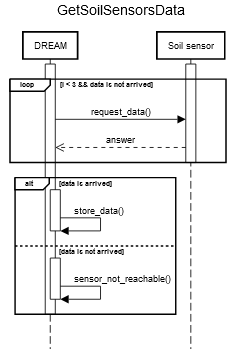
\includegraphics[scale=0.75]{sequence_diagrams/GetSoilSensorsData}
    \caption{Sequence diagram for the GetSoilSensorsData use case}
\end{figure}


%%%%%%%%%%%%%%%%%%%%%%%%%%%%TABLE 8%%%%%%%%%%%%%%%%%%%%%%%

\centering
\begin{longtable}{|p{3.5cm}|m{8cm}|}
 \hline
 \multicolumn{2}{|c|}{\cellcolor{white}\emph{USE CASE 8}} \\
  % do not write anything here
 \endfirsthead
 % do not write anything here
 \endhead
 % do not write anything here
 \endfoot
 % do not write anything here
 \endlastfoot
 \hline
 Name & GetWaterIrrigationSystemData\\
 \hline
 Actor & WaterIrrigationSystem\\
 \hline
 Entry condition & A timer has expired.\\
 \hline
 Event flow & \begin{enumerate}
    \item \verb|DREAM| asks the water irrigation system for some data;
    \item the water irrigation system answers with the data;
    \item \verb|DREAM| stores the data in its database.
 \end{enumerate}\\
 \hline
 Exit condition & \verb|DREAM| has stored in its database the data coming from the water irrigation system.\\
 \hline
 Exceptions & \begin{itemize}
     \item In case the water irrigation system is not reachable, \verb|DREAM| stores that the data of the water irrigation system at that time is not available because "the water irrigation system is not reachable".
 \end{itemize}\\
 \hline
 Special requirements &\begin{itemize}
     \item The water irrigation system must answer in less than 5 seconds;
     \item \verb|DREAM| must try to contact the sensor 3 times before giving up.
 \end{itemize}\\
 \hline
\end{longtable}
\begin{figure}[H]
    \centering
    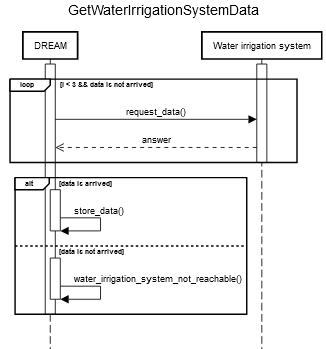
\includegraphics[scale=0.75]{sequence_diagrams/GetWaterIrrigationSystemData}
    \caption{Sequence diagram for the GetWaterIrrigationSystemData use case}
\end{figure}


%%%%%%%%%%%%%%%%%%%%%%%%%%%%TABLE 9%%%%%%%%%%%%%%%%%%%%%%%

\centering
\begin{longtable}{|p{3.5cm}|m{8cm}|}
 \hline
 \multicolumn{2}{|c|}{\cellcolor{white}\emph{USE CASE 9}} \\
  % do not write anything here
 \endfirsthead
 % do not write anything here
 \endhead
 % do not write anything here
 \endfoot
 % do not write anything here
 \endlastfoot
 \hline
 Name & VisualizeAggregateData\\
 \hline
 Actor & PolicyMaker\\
 \hline
 Entry condition & A policy maker accesses the platform and enters the \emph{Aggregate Data} section.\\
 \hline
 Event flow & \begin{enumerate}
    \item The policy maker accesses the system;
    \item the policy maker selects the \emph{Aggregate Data} menu item;
    \item the policy maker chooses the date range they wish to analyze;
    \item \verb|DREAM| generates aggregate statistics for all areas in the database;
    \item \verb|DREAM| shows the data to the user.
 \end{enumerate}\\
 \hline
 Exit condition & The user finishes analyzing the data.\\
 \hline
 Exceptions & \begin{itemize}
     \item If the system has not yet collected any data for the specified period, a warning is returned.
 \end{itemize}\\
 \hline
 Special requirements &\begin{itemize}
     \item The data generation must be completed in less than 3 seconds.
 \end{itemize}\\
 \hline
\end{longtable}

\begin{figure}[H]
    \centering
	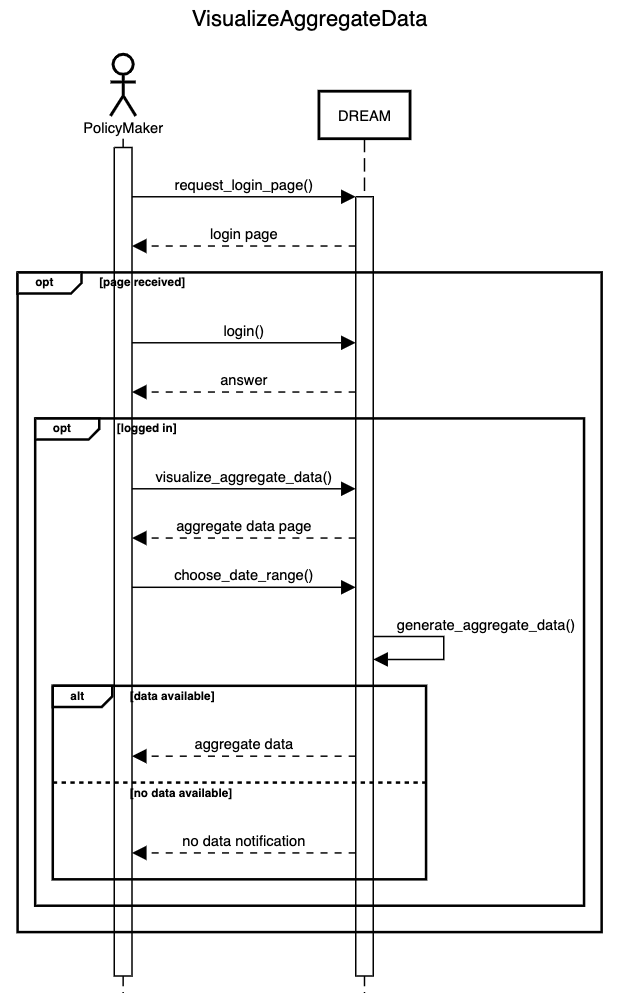
\includegraphics[scale=0.5]{sequence_diagrams/VisualizeAggregateData}
    \caption{Sequence diagram for the VisualizeAggregateData use case}
\end{figure}


%%%%%%%%%%%%%%%%%%%%%%%%%%%%TABLE 10%%%%%%%%%%%%%%%%%%%%%%%

\centering
\begin{longtable}{|p{3.5cm}|m{8cm}|}
 \hline
 \multicolumn{2}{|c|}{\cellcolor{white}\emph{USE CASE 10}} \\
  % do not write anything here
 \endfirsthead
 % do not write anything here
 \endhead
 % do not write anything here
 \endfoot
 % do not write anything here
 \endlastfoot
 \hline
 Name & VisualizeBestFarmers\\
 \hline
 Actor & Agronomist\\
 \hline
 Entry condition & An agronomist accesses the platform and enters the \emph{Farms} section.\\
 \hline
 Event flow & \begin{enumerate}
    \item The agronomist accesses the system;
    \item the agronomist selects the \emph{Farms} menu item;
    \item optionally, the agronomist chooses how the farms should be ranked (e.g. most productive, most resilient to bad weather, ...);
    \item \verb|DREAM| shows a list of the best farms ordered according to the selected parameter.
 \end{enumerate}\\
 \hline
 Exit condition & The user finishes analyzing the data.\\
 \hline
 Exceptions & \begin{itemize}
     \item If the system has not yet collected any data in the agronomist's area, a warning is shown.
 \end{itemize}\\
 \hline
 Special requirements &\begin{itemize}
     \item The data must be shown in less than 1 second.
 \end{itemize}\\
 \hline
\end{longtable}

\begin{figure}[H]
    \centering
	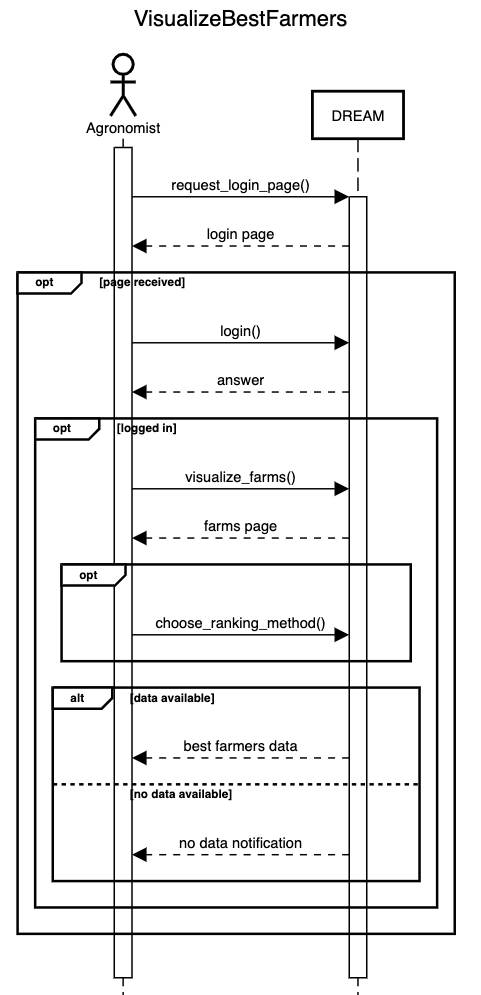
\includegraphics[scale=0.5]{sequence_diagrams/VisualizeBestFarmers}
    \caption{Sequence diagram for the VisualizeBestFarmers use case}
\end{figure}

%%%%%%%%%%%%%%%%%%%%%%%%%%%%TABLE 11%%%%%%%%%%%%%%%%%%%%%%%

\centering
\begin{longtable}{|p{3.5cm}|m{8cm}|}
 \hline
 \multicolumn{2}{|c|}{\cellcolor{white}\emph{USE CASE 11}} \\
  % do not write anything here
 \endfirsthead
 % do not write anything here
 \endhead
 % do not write anything here
 \endfoot
 % do not write anything here
 \endlastfoot
 \hline
 Name & VisualizeForecasts\\
 \hline
 Actor & Agronomist\\
 \hline
 Entry condition & An agronomist accesses the platform and enters the \emph{Weather Forecasts} section.\\
 \hline
 Event flow & \begin{enumerate}
    \item The agronomist accesses the system;
    \item the agronomist selects the \emph{Weather Forecasts} menu item;
    \item the agronomist chooses the date for which forecasts should be shown;
    \item \verb|DREAM| connects to the Telengana government website to fetch forecasts for the chosen date;
    \item \verb|DREAM| shows a map with the forecast.
 \end{enumerate}\\
 \hline
 Exit condition & The user finishes analyzing the data.\\
 \hline
 Exceptions & \begin{itemize}
     \item If the Telengana government website is currently unreachable, an error is shown to the user.
     \item If no weather data is available for the chosen date, an error is shown to the user.
 \end{itemize}\\
 \hline
 Special requirements &\begin{itemize}
     \item The Telengana government website must serve requests in less than 5 seconds;
     \item The Telengana government website is assumed not to change in a backwards-incompatible manner without notice.
 \end{itemize}\\
 \hline
\end{longtable}

\begin{figure}[H]
    \centering
	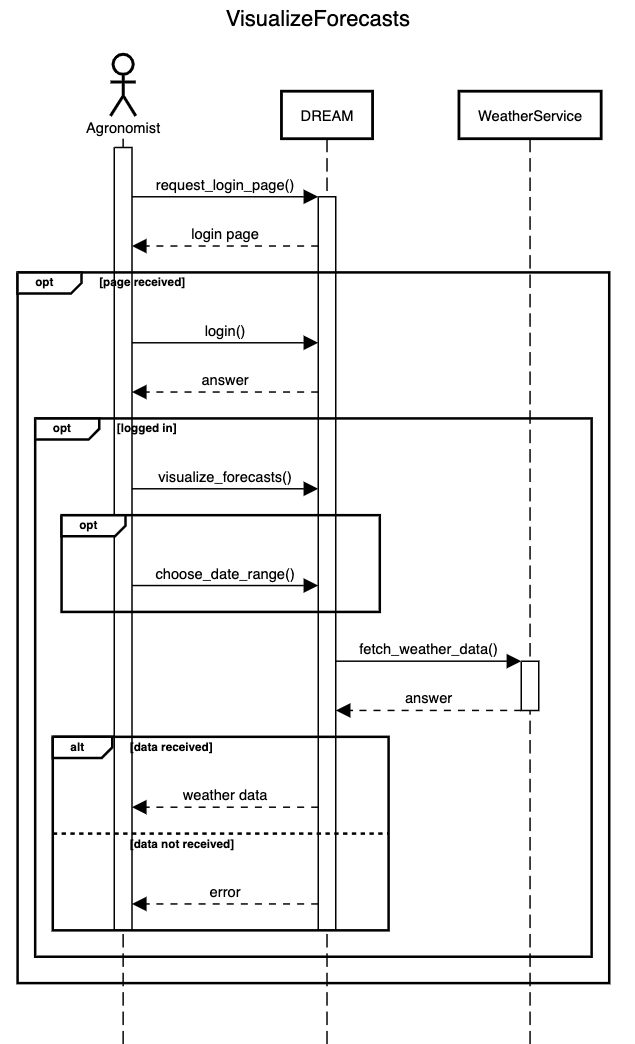
\includegraphics[scale=0.5]{sequence_diagrams/VisualizeForecasts}
    \caption{Sequence diagram for the VisualizeForecasts use case}
\end{figure}
%%%%%%%%%%%%%%%%%%%%%%%%%%%%TABLE 12%%%%%%%%%%%%%%%%%%%%%%%

\centering
\begin{longtable}{|p{3.5cm}|m{8cm}|}
 \hline
 \multicolumn{2}{|c|}{\cellcolor{white}\emph{USE CASE 12}} \\
  % do not write anything here
 \endfirsthead
 % do not write anything here
 \endhead
 % do not write anything here
 \endfoot
 % do not write anything here
 \endlastfoot
 \hline
 Name & VisualizeFarmerSuggestions\\
 \hline
 Actor & Farmer\\
 \hline
 Entry condition & A farmer wants to check if there are any suggestions for them.\\
 \hline
 Event flow & \begin{enumerate}
    \item The farmer accesses the system;
    \item the farmer accesses the \emph{Suggestions} section;
    \item \verb|DREAM| automatically shows suggestions for the farmer.
 \end{enumerate}\\
 \hline
 Exit condition & The farmer views the list of suggestions.\\
 \hline
 Exceptions & \begin{itemize}
     \item If there are no suggestions for the farmer, a notice is shown.
 \end{itemize}\\
 \hline
 Special requirements & None.\\
 \hline
\end{longtable}
\newpage
%%%%%%%%%%%%%%%%%%%%%%%%%%%%TABLE 13%%%%%%%%%%%%%%%%%%%%%%%

\centering
\begin{longtable}{|p{3.5cm}|m{8cm}|}
 \hline
 \multicolumn{2}{|c|}{\cellcolor{white}\emph{USE CASE 13}} \\
  % do not write anything here
 \endfirsthead
 % do not write anything here
 \endhead
 % do not write anything here
 \endfoot
 % do not write anything here
 \endlastfoot
 \hline
 Name & GetWeatherForecasts\\
 \hline
 Actor & OuterWeatherSource\\
 \hline
 Entry condition & Either (a) a user requests weather data; or (b) \verb|DREAM| needs to access weather information for statistical purposes.\\
 \hline
 Event flow & \begin{enumerate}
    \item \verb|DREAM| connects to the Telengana government website to fetch the required forecasts;
    \item The data is stored and analyzed as needed.
 \end{enumerate}\\
 \hline
 Exit condition & The weather forecast data is collected by the system.\\
 \hline
 Exceptions & \begin{itemize}
     \item If the Telengana government website is currently unreachable, the process is aborted and an error is returned.
 \end{itemize}\\
 \hline
 Special requirements &\begin{itemize}
     \item The Telengana government website must serve requests in less than 5 seconds;
     \item The Telengana government website is assumed not to change in a backwards-incompatible manner without notice.
 \end{itemize}\\
 \hline
\end{longtable}
\newpage
\raggedright
\subsection{Performance Requirements}
This section is dedicated to “specify both the static and the dynamic numerical requirements placed on the software or on human interaction with the software as a whole”\footnote{IEEE 29148-2018 Requirements engineering, section 9.6.14}.
Static numerical requirements:
\begin{itemize}
\item according to the estimates\footnote{professor Jayashankar Telangana state agricultural university}, Telengana has a population of 36 millions of people and a total number of farm holdings equal to 55.54 lakhs, namely more or less 5 555 400 people in Telangana are farmers; assuming that all of them are potential users of \verb|DREAM|, it must support at least 5.7 million non-simultaneously connected terminals, since also the agronomists and policy makers shall be allowed to access the system;
\item given the huge number of (possible) users and the purpose of the system, \verb|DREAM| must be able to support at least 10\% of the total number of users simultaneously; this requirement is more important than speed performances;
\item all the weather reports and forecasts are not directly stored on \verb|DREAM|; nevertheless, \verb|DREAM| must store all the sensors and water irrigation system data as well as the users data and the forums data. 
We can assume that the system stores 1KB of personal information for each user:
\[ usersData = 5.7 * 10^6 users * 1 KB \approx 5.7 GB \]
Assuming an average of 1000 posts a day, the data required for 1 year is (assumption: 1KB for each post, no images allowed):
\[forumData = 1 KB * 1000 posts/day * 365 days/year \approx 365 MB \]
Plus 32 bytes for each sensor measurement (16 bytes to recognize the sensor, 8 bytes for the timestamp and 8 bytes for the soil moisture value; we estimate 10 000 humidity sensors in Telangana whose data is retrieved 3 times a day):
\[sensorsData = 32 B * 10 000 sensors * 3 measurements/day * 365 days/year \approx 350 MB \]
Plus 32B additional bytes for each farmer because of the water irrigation system:
\[waterIrrigationSystemData = 32 B * 12 measurements/year * 5.5 * 10^6 farmers \approx 2 GB \]
Plus 1KB for each production report stored in \verb|DREAM| (assuming that each farmer uploads the production data once for each month):
\[productionData = 1 KB * 12 reports/year * 5.5 * 10^6 farmers \approx 66 GB \]
Plus some additional data for the daily plans, that we can neglect because of the small number of agronomists with regards to the number of farmers.\\
This means that the amount of information to be effectively stored must be in the rank of:
\[totalData = \sum_{i=1}^{5} data[i] \approx 74 GB \]
In this calculation is not considered all the space required to perform analysis over the stored data and the data accessed over the Telangana's government website (namely, weather reports and forecasts). Therefore, we can assume that a database of $100 GB$ can suffice for the first year.
\end{itemize}
Dynamic numerical requirements:
\begin{itemize}
\item all the transactions must be processed in less than 3 seconds (as said before, \verb|DREAM| does not require strict temporal requirements);
\item the number of transactions the system has to process during peak workload conditions is in the order of $10^4$.
\end{itemize}

\subsection{Design Constraints}
In this section we “specify constraints on the system design imposed by external standards, regulatory requirements or project limitations”\footnote{IEEE 29148-2018 Requirements engineering, section 9.6.16}.
\subsubsection{Standard compliance}
\verb|DREAM| stores personal data of the users, like name, surname, job, location of the farm (if he is a farmer) … . Therefore, this data must be treated according to the privacy regulations in India.
\subsubsection{Hardware limitation}
Since \verb|DREAM| is a webapp, every device with a browser recent enough can be used to access the system. \verb|DREAM| does not impose any constraint on the sensors and the water irrigation system, as long as the central hub uses a standardized protocol for communication.
\subsubsection{Any other constraint}
No any other specific constraint is required.
\subsection{Software System Attributes}
In this section a list of required attributes of the system is provided.
\subsubsection{Reliability}
\verb|DREAM| is not a critical system, therefore some limited failures cannot create big problems. For example, an error when accessing the Telengana’s website or a failure during the generation of the daily plan can be easily solved just by re-starting the process.
\subsubsection{Availability}
The system is not critical, as already said, therefore some periods of inactivity are allowed. Because all the tasks it performs are not critical, small periods of inactivity do not create many problems. For instance, when a farmer needs to ask for help, he could make the request even the following day. Another example is the access to the humidity sensors: data of today could be accessed even tomorrow since they are stored in Telengana’s website as well. A final example is about the proposal of a schedule plan; agronomists can wait some time before retrieving it. 
We can impose that \verb|DREAM| must not be unavailable for more than 1 day per month.
\subsubsection{Security}
The only information that needs to be protected is the personal data of the users. Therefore, \verb|DREAM| has to assure data privacy. This can be done by ensuring that all connections are established securely via HTTPS.
\subsubsection{Maintainability}
The system must be designed in order to facilitate maintainability. Every functionality implemented must be well documented. The system must be decomposed in a certain number of modules to limit the complexity and to make the development process more efficient. The main goal is that each module is coherent and can be (internally) modified without affecting other modules and without changing its interface.
\subsubsection{Portability}
Since \verb|DREAM| is a webapp, it does not have strict requirements on the underlying operating system or hardware used. The website will be developed using an interpreted language with a widely available interpreter.

\section{Formal analysis using Alloy}

\begin{minted}{alloy}
open util/integer
open util/ordering [DateTime] // adds ordering to DateTime objects

/**** SIGNATURES ****/
sig DateTime {}
abstract sig User {}
sig Farmer extends User {
	farm: one Farm
}
sig Agronomist extends User {
	// For the purposes of this Alloy specification,
	// we assume all Agronomists have already selected their area.
	area: one Area
}
sig Farm {
	area: one Area,
}
sig DailyPlan {
	agronomist: one Agronomist,
	fromDateTime: one DateTime,
	toDateTime: one DateTime
}
sig FarmVisit {
	dailyPlan: one DailyPlan,
	farm: one Farm,
	dateTime: one DateTime
}
sig Area {}
sig ProductionData {
	farm: one Farm,
	fromDateTime: one DateTime,
	toDateTime: one DateTime,
	volume: one Int
}
sig ProductionIssue {
	productionData: one ProductionData
}

/**** FUNCTIONS ****/
fun FarmVisits[fx: Farm]: set FarmVisit {
	{ fv: FarmVisit | fv.farm = fx }
}

fun FarmerVisits[f: Farmer]: set FarmVisit {
	FarmVisits[f.farm]
}

fun FarmVisitAgronomist[fv: FarmVisit]: one Agronomist {
	fv.dailyPlan.agronomist
}

fun AgronomistVisits[a: Agronomist]: set FarmVisit {
	{ fv: FarmVisit | FarmVisitAgronomist[fv] = a }
}

fun FarmerIssues[f: Farmer]: set ProductionIssue {
	{ i: ProductionIssue | i.productionData.farm = f.farm }
}

fun AgronomistDailyPlans[a: Agronomist]: set DailyPlan {
	{ p: DailyPlan | p.agronomist = a }
}

/**** FACTS ****/
// Every farm has exactly one farmer
fact { all fx: Farm | one f: Farmer | f.farm = fx }

// All areas have at least one agronomist
fact { all a: Area | some agr: Agronomist | agr.area = a }

// All areas have at least one farmer
fact { all a: Area | some f: Farmer | f.farm.area = a }

// All farms are visited at least twice
// (Note: For the purposes of this specification, we assume all visits
// in the generated world happen in the same year)
fact { all fx: Farm | (let v = FarmVisits[fx] | #v >= 2) }

// Every Daily Plan has at least one visit
fact { all p: DailyPlan | some v: FarmVisit | v.dailyPlan = p }

// Daily Plan dates are consistent
fact { all p: DailyPlan | lt[p.fromDateTime, p.toDateTime] }

// Farm Visit dates are consistent with their daily plan
fact {
    all fv: FarmVisit | (
        gte[fv.dateTime, fv.dailyPlan.fromDateTime] and
        lte[fv.dateTime, fv.dailyPlan.toDateTime]
    )
}

// Agronomists only visit farms in their area
fact { all fv: FarmVisit | fv.farm.area = FarmVisitAgronomist[fv].area }

// Farmers who had more production issues are visited more often
// (relative to other farmers in their area)
fact {
    all disj f1: Farmer, f2: Farmer |
        (f1.farm.area = f2.farm.area and #FarmerIssues[f1] > #FarmerIssues[f2])
        implies
        #FarmerVisits[f1] >= #FarmerVisits[f2]
}

// Agronomists in the same area "split" their work,
// i.e no agronomist does more than twice
// the number of visits of any of their colleagues.
fact {
    all disj a1: Agronomist, a2: Agronomist | (
        a1.area = a2.area
        implies
        #AgronomistVisits[a1] <= mul[2, #AgronomistVisits[a2]]
    )
}

// Production volume is nonnegative
fact { all d: ProductionData | d.volume >= 0 }

// Production datetimes are consistent
fact { all d: ProductionData | lt[d.fromDateTime, d.toDateTime] }

/**** PREDICATES (WORLD GENERATION) ****/
pred WorldSimple {
	#Area = 1
	#Farmer = 1
	#Agronomist = 1
}

pred WorldManyAgronomists {
	#Area = 1
	#Farmer = 2
	#Agronomist = 5
	#FarmVisit = 5
}

pred WorldFarmersIssues {
	#Area = 1
	#Farmer = 2
	#Agronomist = 2
	#ProductionData = 2
	#ProductionIssue = 5
	#FarmVisit = 5
	// Every farmer had at least one issue
	all f: Farmer | #FarmerIssues[f] >= 1
}

/**** ASSERTIONS ****/
// All farmers have a "reference" agronomist
//(i.e. the agronomist they can contact via DREAM)
assert FarmerReferenceAgronomists {
	all f: Farmer | some agr: Agronomist | f.farm.area = agr.area
}

// All agronomists have at least one daily plan
assert AgronomistDailyPlans {
	all a: Agronomist | #AgronomistDailyPlans[a] > 0
}

// All agronomists visit some farms
assert AgronomistFarmVisits {
	all a: Agronomist | #AgronomistVisits[a] > 0
}

/**** EXECUTION ****/
check FarmerReferenceAgronomists for 5
check AgronomistFarmVisits for 5
check AgronomistDailyPlans for 5
run WorldSimple for 5
run WorldManyAgronomists for 10
run WorldFarmersIssues for 5
\end{minted}
\section{Effort spent}
\section{References}
\end{document}

